% Standalone ACM manuscript: bibliography and evidence-backed plots are embedded.
% Generated figure blocks are refreshed by experiments/build_paper_figures.py.
\documentclass[sigconf,screen,nonacm]{acmart}
\usepackage{amsmath}
\usepackage{pgfplots}
\usepgfplotslibrary{groupplots}
\usetikzlibrary{arrows.meta,positioning}
\pgfplotsset{compat=1.18}
\setcopyright{none}
\settopmatter{printacmref=false,printfolios=true}
\citestyle{acmnumeric}
\newcommand{\E}{\mathbb{E}}
\newcommand{\Prob}{\mathbb{P}}
\newcommand{\ind}{\mathbf{1}}
\newcommand{\pp}{\boldsymbol{p}}
\newcommand{\avec}{\boldsymbol{a}}
\newcommand{\Vvec}{\boldsymbol{v}}
\newcommand{\Mvec}{\boldsymbol{m}}
\newcommand{\Wvec}{\boldsymbol{w}}
\newcommand{\Core}{j_0}
\newtheorem{result}{Theorem}[section]
\newtheorem{claim}[result]{Proposition}
\newtheorem{fact}[result]{Lemma}
\definecolor{inkblue}{RGB}{32,82,128}
\definecolor{warmred}{RGB}{177,56,46}
\definecolor{leafgreen}{RGB}{42,118,86}
\pgfplotsset{every axis/.append style={font=\small,
  tick label style={font=\footnotesize},label style={font=\small},
  legend style={font=\footnotesize,draw=none},grid=major,
  grid style={gray!15},axis line style={gray!65}}}

% BEGIN GENERATED FIGURES
\newcommand{\PaperCostCurves}{%
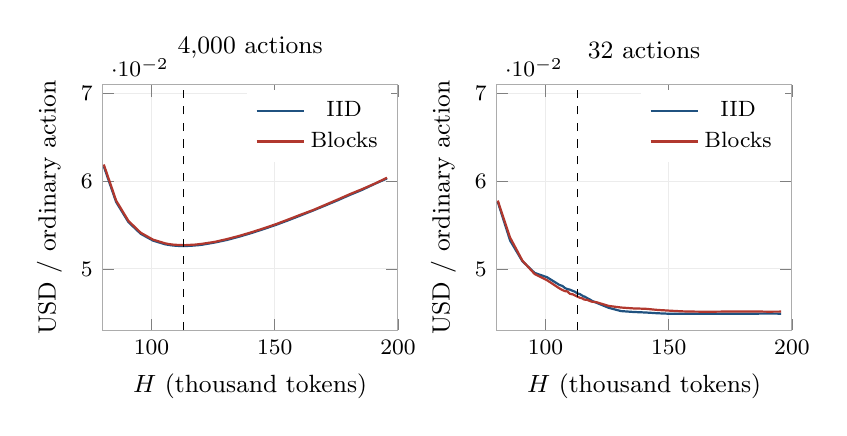
\begin{tikzpicture}
\begin{groupplot}[group style={group size=2 by 1,horizontal sep=1.25cm},
  width=.44\textwidth,height=4.7cm,xlabel={$H$ (thousand tokens)},
  ylabel={USD / ordinary action},xmin=80,xmax=200,
  legend style={at={(.98,.98)},anchor=north east}]
\nextgroupplot[title={4,000 actions},ymin=.043,ymax=.071]
\addplot[inkblue,thick] coordinates {(80.588,0.06170189) (85.588,0.057638643) (90.588,0.055340336) (95.588,0.054006682) (100.588,0.053229621) (105.588,0.052803455) (106.848,0.052746026) (107.848,0.052697994) (108.848,0.052670973) (109.848,0.052645006) (110.588,0.052634412) (110.848,0.052624738) (111.848,0.052616299) (112.848,0.052618706) (113.848,0.052609099) (114.848,0.052629544) (115.4275,0.05263323) (115.588,0.052636572) (115.848,0.052640214) (116.848,0.052661184) (117.848,0.052684165) (118.848,0.052704606) (120.588,0.052767436) (125.588,0.053009792) (130.588,0.053307333) (135.588,0.053682442) (140.588,0.054099978) (145.588,0.054554597) (150.588,0.055036436) (155.588,0.055558915) (160.588,0.056105806) (165.588,0.056663617) (170.588,0.057242801) (175.588,0.057832395) (180.588,0.058452213) (185.588,0.059032235) (190.588,0.059701796) (195.588,0.060319128)};
\addlegendentry{IID}
\addplot[warmred,thick] coordinates {(80.588,0.061906929) (85.588,0.057802237) (90.588,0.055478924) (95.588,0.054125474) (100.588,0.053339061) (105.588,0.05291191) (106.848,0.052848825) (107.848,0.05280306) (108.848,0.052771516) (109.848,0.052757432) (110.588,0.052729266) (110.848,0.05272967) (111.848,0.052721455) (112.848,0.052718783) (113.848,0.05271681) (114.848,0.052723815) (115.4275,0.052737866) (115.588,0.052742123) (115.848,0.052749721) (116.848,0.052764503) (117.848,0.05277929) (118.848,0.052813143) (120.588,0.0528703) (125.588,0.053084305) (130.588,0.053405496) (135.588,0.053770193) (140.588,0.054187061) (145.588,0.054636626) (150.588,0.055118042) (155.588,0.055650508) (160.588,0.056195195) (165.588,0.056716993) (170.588,0.057315461) (175.588,0.057920391) (180.588,0.05853918) (185.588,0.059113359) (190.588,0.059729347) (195.588,0.060400825)};
\addlegendentry{Blocks}
\addplot[black,dashed,forget plot] coordinates {(112.848,.043)(112.848,.071)};
\nextgroupplot[title={32 actions},ymin=.043,ymax=.071]
\addplot[inkblue,thick] coordinates {(80.588,0.057647339) (85.588,0.053242696) (90.588,0.050877033) (95.588,0.049542258) (100.588,0.049054896) (105.588,0.048183981) (106.848,0.048055974) (107.848,0.047829706) (108.848,0.047696313) (109.848,0.047639296) (110.588,0.047550367) (110.848,0.047519439) (111.848,0.047411051) (112.848,0.047217476) (113.848,0.047139308) (114.848,0.046971531) (115.4275,0.046855603) (115.588,0.046853776) (115.848,0.046849395) (116.848,0.046674765) (117.848,0.046537692) (118.848,0.046364445) (120.588,0.046150656) (125.588,0.045573322) (130.588,0.04519576) (135.588,0.045094616) (140.588,0.045033172) (145.588,0.044944271) (150.588,0.044886423) (155.588,0.04488897) (160.588,0.044893985) (165.588,0.044894658) (170.588,0.044898673) (175.588,0.044891814) (180.588,0.044900454) (185.588,0.044900454) (190.588,0.044911637) (195.588,0.044899189)};
\addlegendentry{IID}
\addplot[warmred,thick] coordinates {(80.588,0.057795875) (85.588,0.053580723) (90.588,0.050947456) (95.588,0.049415465) (100.588,0.048714695) (105.588,0.047790285) (106.848,0.047592479) (107.848,0.047470605) (108.848,0.047438365) (109.848,0.047170067) (110.588,0.047121591) (110.848,0.047136736) (111.848,0.046986383) (112.848,0.046849507) (113.848,0.046721826) (114.848,0.04664769) (115.4275,0.046541752) (115.588,0.046534563) (115.848,0.046502403) (116.848,0.046480923) (117.848,0.046361484) (118.848,0.046260241) (120.588,0.046212052) (125.588,0.045785839) (130.588,0.04560115) (135.588,0.045500375) (140.588,0.045457989) (145.588,0.045322254) (150.588,0.045238564) (155.588,0.045164063) (160.588,0.045134522) (165.588,0.045122133) (170.588,0.045133307) (175.588,0.045145817) (180.588,0.045149938) (185.588,0.045142148) (190.588,0.045128165) (195.588,0.045135893)};
\addlegendentry{Blocks}
\addplot[black,dashed,forget plot] coordinates {(112.848,.043)(112.848,.071)};
\end{groupplot}
\end{tikzpicture}}
\newcommand{\PaperPricePhase}{%
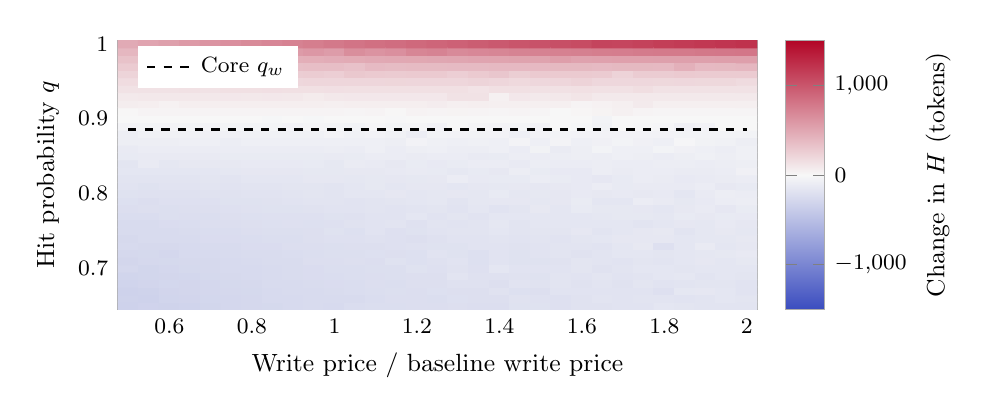
\begin{tikzpicture}
\begin{axis}[width=.80\textwidth,height=5cm,
  xlabel={Write price / baseline write price},ylabel={Hit probability $q$},
  xmin=.475,xmax=2.025,ymin=.645,ymax=1.005,
  colormap={signed}{rgb(0cm)=(.23,.30,.75);rgb(1cm)=(.97,.97,.97);
    rgb(2cm)=(.70,.02,.15)},point meta min=-1500,point meta max=1500,
  colorbar,colorbar style={ylabel={Change in $H$ (tokens)},font=\footnotesize},
  grid=none,legend style={at={(.03,.98)},anchor=north west,fill=white}]
\addplot[matrix plot*,mesh/cols=31,point meta=explicit,forget plot]
table[x=factor,y=q,meta=delta,row sep=\\] {
factor q delta\\
0.5 0.65 -325\\
0.55 0.65 -315\\
0.6 0.65 -320\\
0.65 0.65 -310\\
0.7 0.65 -295\\
0.75 0.65 -280\\
0.8 0.65 -275\\
0.85 0.65 -270\\
0.9 0.65 -260\\
0.95 0.65 -245\\
1 0.65 -255\\
1.05 0.65 -230\\
1.1 0.65 -225\\
1.15 0.65 -225\\
1.2 0.65 -220\\
1.25 0.65 -220\\
1.3 0.65 -210\\
1.35 0.65 -220\\
1.4 0.65 -220\\
1.45 0.65 -190\\
1.5 0.65 -190\\
1.55 0.65 -200\\
1.6 0.65 -185\\
1.65 0.65 -185\\
1.7 0.65 -180\\
1.75 0.65 -175\\
1.8 0.65 -155\\
1.85 0.65 -160\\
1.9 0.65 -170\\
1.95 0.65 -165\\
2 0.65 -170\\
0.5 0.66 -320\\
0.55 0.66 -325\\
0.6 0.66 -305\\
0.65 0.66 -300\\
0.7 0.66 -285\\
0.75 0.66 -280\\
0.8 0.66 -275\\
0.85 0.66 -260\\
0.9 0.66 -255\\
0.95 0.66 -245\\
1 0.66 -245\\
1.05 0.66 -245\\
1.1 0.66 -230\\
1.15 0.66 -220\\
1.2 0.66 -220\\
1.25 0.66 -225\\
1.3 0.66 -205\\
1.35 0.66 -210\\
1.4 0.66 -210\\
1.45 0.66 -185\\
1.5 0.66 -195\\
1.55 0.66 -200\\
1.6 0.66 -185\\
1.65 0.66 -170\\
1.7 0.66 -180\\
1.75 0.66 -165\\
1.8 0.66 -170\\
1.85 0.66 -180\\
1.9 0.66 -170\\
1.95 0.66 -150\\
2 0.66 -160\\
0.5 0.67 -325\\
0.55 0.67 -320\\
0.6 0.67 -300\\
0.65 0.67 -290\\
0.7 0.67 -280\\
0.75 0.67 -275\\
0.8 0.67 -270\\
0.85 0.67 -260\\
0.9 0.67 -250\\
0.95 0.67 -250\\
1 0.67 -240\\
1.05 0.67 -230\\
1.1 0.67 -225\\
1.15 0.67 -215\\
1.2 0.67 -220\\
1.25 0.67 -205\\
1.3 0.67 -210\\
1.35 0.67 -210\\
1.4 0.67 -185\\
1.45 0.67 -205\\
1.5 0.67 -210\\
1.55 0.67 -180\\
1.6 0.67 -175\\
1.65 0.67 -180\\
1.7 0.67 -175\\
1.75 0.67 -175\\
1.8 0.67 -200\\
1.85 0.67 -145\\
1.9 0.67 -140\\
1.95 0.67 -155\\
2 0.67 -175\\
0.5 0.68 -310\\
0.55 0.68 -300\\
0.6 0.68 -285\\
0.65 0.68 -290\\
0.7 0.68 -280\\
0.75 0.68 -270\\
0.8 0.68 -265\\
0.85 0.68 -250\\
0.9 0.68 -250\\
0.95 0.68 -240\\
1 0.68 -235\\
1.05 0.68 -230\\
1.1 0.68 -220\\
1.15 0.68 -225\\
1.2 0.68 -210\\
1.25 0.68 -210\\
1.3 0.68 -195\\
1.35 0.68 -195\\
1.4 0.68 -210\\
1.45 0.68 -180\\
1.5 0.68 -185\\
1.55 0.68 -170\\
1.6 0.68 -185\\
1.65 0.68 -170\\
1.7 0.68 -185\\
1.75 0.68 -160\\
1.8 0.68 -175\\
1.85 0.68 -170\\
1.9 0.68 -160\\
1.95 0.68 -160\\
2 0.68 -175\\
0.5 0.69 -305\\
0.55 0.69 -295\\
0.6 0.69 -290\\
0.65 0.69 -285\\
0.7 0.69 -270\\
0.75 0.69 -265\\
0.8 0.69 -260\\
0.85 0.69 -250\\
0.9 0.69 -240\\
0.95 0.69 -235\\
1 0.69 -230\\
1.05 0.69 -225\\
1.1 0.69 -220\\
1.15 0.69 -215\\
1.2 0.69 -210\\
1.25 0.69 -210\\
1.3 0.69 -170\\
1.35 0.69 -195\\
1.4 0.69 -195\\
1.45 0.69 -185\\
1.5 0.69 -190\\
1.55 0.69 -165\\
1.6 0.69 -175\\
1.65 0.69 -160\\
1.7 0.69 -175\\
1.75 0.69 -170\\
1.8 0.69 -150\\
1.85 0.69 -145\\
1.9 0.69 -165\\
1.95 0.69 -155\\
2 0.69 -160\\
0.5 0.7 -275\\
0.55 0.7 -295\\
0.6 0.7 -280\\
0.65 0.7 -270\\
0.7 0.7 -265\\
0.75 0.7 -260\\
0.8 0.7 -255\\
0.85 0.7 -245\\
0.9 0.7 -240\\
0.95 0.7 -235\\
1 0.7 -225\\
1.05 0.7 -225\\
1.1 0.7 -215\\
1.15 0.7 -215\\
1.2 0.7 -190\\
1.25 0.7 -200\\
1.3 0.7 -185\\
1.35 0.7 -200\\
1.4 0.7 -150\\
1.45 0.7 -180\\
1.5 0.7 -175\\
1.55 0.7 -180\\
1.6 0.7 -160\\
1.65 0.7 -185\\
1.7 0.7 -165\\
1.75 0.7 -155\\
1.8 0.7 -155\\
1.85 0.7 -160\\
1.9 0.7 -150\\
1.95 0.7 -155\\
2 0.7 -150\\
0.5 0.71 -290\\
0.55 0.71 -275\\
0.6 0.71 -270\\
0.65 0.71 -265\\
0.7 0.71 -265\\
0.75 0.71 -255\\
0.8 0.71 -250\\
0.85 0.71 -240\\
0.9 0.71 -240\\
0.95 0.71 -220\\
1 0.71 -220\\
1.05 0.71 -210\\
1.1 0.71 -220\\
1.15 0.71 -190\\
1.2 0.71 -205\\
1.25 0.71 -195\\
1.3 0.71 -175\\
1.35 0.71 -205\\
1.4 0.71 -175\\
1.45 0.71 -190\\
1.5 0.71 -190\\
1.55 0.71 -185\\
1.6 0.71 -160\\
1.65 0.71 -165\\
1.7 0.71 -180\\
1.75 0.71 -160\\
1.8 0.71 -170\\
1.85 0.71 -155\\
1.9 0.71 -140\\
1.95 0.71 -155\\
2 0.71 -135\\
0.5 0.72 -275\\
0.55 0.72 -270\\
0.6 0.72 -280\\
0.65 0.72 -260\\
0.7 0.72 -260\\
0.75 0.72 -250\\
0.8 0.72 -240\\
0.85 0.72 -240\\
0.9 0.72 -230\\
0.95 0.72 -225\\
1 0.72 -215\\
1.05 0.72 -215\\
1.1 0.72 -205\\
1.15 0.72 -210\\
1.2 0.72 -205\\
1.25 0.72 -180\\
1.3 0.72 -190\\
1.35 0.72 -205\\
1.4 0.72 -175\\
1.45 0.72 -190\\
1.5 0.72 -180\\
1.55 0.72 -165\\
1.6 0.72 -185\\
1.65 0.72 -165\\
1.7 0.72 -150\\
1.75 0.72 -150\\
1.8 0.72 -160\\
1.85 0.72 -155\\
1.9 0.72 -145\\
1.95 0.72 -135\\
2 0.72 -125\\
0.5 0.73 -260\\
0.55 0.73 -265\\
0.6 0.73 -265\\
0.65 0.73 -255\\
0.7 0.73 -245\\
0.75 0.73 -245\\
0.8 0.73 -235\\
0.85 0.73 -235\\
0.9 0.73 -220\\
0.95 0.73 -220\\
1 0.73 -215\\
1.05 0.73 -210\\
1.1 0.73 -210\\
1.15 0.73 -200\\
1.2 0.73 -195\\
1.25 0.73 -190\\
1.3 0.73 -190\\
1.35 0.73 -175\\
1.4 0.73 -180\\
1.45 0.73 -185\\
1.5 0.73 -175\\
1.55 0.73 -170\\
1.6 0.73 -165\\
1.65 0.73 -180\\
1.7 0.73 -150\\
1.75 0.73 -130\\
1.8 0.73 -200\\
1.85 0.73 -155\\
1.9 0.73 -115\\
1.95 0.73 -155\\
2 0.73 -140\\
0.5 0.74 -265\\
0.55 0.74 -245\\
0.6 0.74 -250\\
0.65 0.74 -245\\
0.7 0.74 -235\\
0.75 0.74 -235\\
0.8 0.74 -230\\
0.85 0.74 -225\\
0.9 0.74 -225\\
0.95 0.74 -210\\
1 0.74 -200\\
1.05 0.74 -200\\
1.1 0.74 -195\\
1.15 0.74 -200\\
1.2 0.74 -210\\
1.25 0.74 -195\\
1.3 0.74 -175\\
1.35 0.74 -175\\
1.4 0.74 -170\\
1.45 0.74 -175\\
1.5 0.74 -170\\
1.55 0.74 -175\\
1.6 0.74 -160\\
1.65 0.74 -155\\
1.7 0.74 -140\\
1.75 0.74 -140\\
1.8 0.74 -140\\
1.85 0.74 -150\\
1.9 0.74 -145\\
1.95 0.74 -145\\
2 0.74 -130\\
0.5 0.75 -250\\
0.55 0.75 -245\\
0.6 0.75 -245\\
0.65 0.75 -240\\
0.7 0.75 -230\\
0.75 0.75 -230\\
0.8 0.75 -220\\
0.85 0.75 -215\\
0.9 0.75 -215\\
0.95 0.75 -210\\
1 0.75 -190\\
1.05 0.75 -205\\
1.1 0.75 -180\\
1.15 0.75 -200\\
1.2 0.75 -190\\
1.25 0.75 -180\\
1.3 0.75 -165\\
1.35 0.75 -165\\
1.4 0.75 -155\\
1.45 0.75 -170\\
1.5 0.75 -160\\
1.55 0.75 -160\\
1.6 0.75 -140\\
1.65 0.75 -165\\
1.7 0.75 -150\\
1.75 0.75 -140\\
1.8 0.75 -130\\
1.85 0.75 -165\\
1.9 0.75 -145\\
1.95 0.75 -130\\
2 0.75 -145\\
0.5 0.76 -250\\
0.55 0.76 -245\\
0.6 0.76 -235\\
0.65 0.76 -230\\
0.7 0.76 -220\\
0.75 0.76 -220\\
0.8 0.76 -210\\
0.85 0.76 -205\\
0.9 0.76 -200\\
0.95 0.76 -205\\
1 0.76 -200\\
1.05 0.76 -185\\
1.1 0.76 -180\\
1.15 0.76 -170\\
1.2 0.76 -195\\
1.25 0.76 -165\\
1.3 0.76 -180\\
1.35 0.76 -165\\
1.4 0.76 -145\\
1.45 0.76 -170\\
1.5 0.76 -155\\
1.55 0.76 -155\\
1.6 0.76 -150\\
1.65 0.76 -155\\
1.7 0.76 -155\\
1.75 0.76 -170\\
1.8 0.76 -150\\
1.85 0.76 -140\\
1.9 0.76 -145\\
1.95 0.76 -125\\
2 0.76 -140\\
0.5 0.77 -230\\
0.55 0.77 -230\\
0.6 0.77 -215\\
0.65 0.77 -220\\
0.7 0.77 -225\\
0.75 0.77 -210\\
0.8 0.77 -205\\
0.85 0.77 -200\\
0.9 0.77 -200\\
0.95 0.77 -200\\
1 0.77 -190\\
1.05 0.77 -195\\
1.1 0.77 -180\\
1.15 0.77 -175\\
1.2 0.77 -155\\
1.25 0.77 -175\\
1.3 0.77 -160\\
1.35 0.77 -180\\
1.4 0.77 -150\\
1.45 0.77 -155\\
1.5 0.77 -150\\
1.55 0.77 -150\\
1.6 0.77 -150\\
1.65 0.77 -145\\
1.7 0.77 -135\\
1.75 0.77 -135\\
1.8 0.77 -145\\
1.85 0.77 -120\\
1.9 0.77 -130\\
1.95 0.77 -120\\
2 0.77 -125\\
0.5 0.78 -220\\
0.55 0.78 -210\\
0.6 0.78 -215\\
0.65 0.78 -210\\
0.7 0.78 -210\\
0.75 0.78 -200\\
0.8 0.78 -195\\
0.85 0.78 -190\\
0.9 0.78 -190\\
0.95 0.78 -185\\
1 0.78 -180\\
1.05 0.78 -175\\
1.1 0.78 -170\\
1.15 0.78 -180\\
1.2 0.78 -165\\
1.25 0.78 -160\\
1.3 0.78 -175\\
1.35 0.78 -150\\
1.4 0.78 -180\\
1.45 0.78 -160\\
1.5 0.78 -130\\
1.55 0.78 -155\\
1.6 0.78 -120\\
1.65 0.78 -135\\
1.7 0.78 -135\\
1.75 0.78 -140\\
1.8 0.78 -155\\
1.85 0.78 -130\\
1.9 0.78 -115\\
1.95 0.78 -140\\
2 0.78 -110\\
0.5 0.79 -205\\
0.55 0.79 -220\\
0.6 0.79 -200\\
0.65 0.79 -200\\
0.7 0.79 -200\\
0.75 0.79 -190\\
0.8 0.79 -190\\
0.85 0.79 -185\\
0.9 0.79 -180\\
0.95 0.79 -170\\
1 0.79 -170\\
1.05 0.79 -180\\
1.1 0.79 -165\\
1.15 0.79 -160\\
1.2 0.79 -155\\
1.25 0.79 -145\\
1.3 0.79 -165\\
1.35 0.79 -145\\
1.4 0.79 -140\\
1.45 0.79 -140\\
1.5 0.79 -145\\
1.55 0.79 -140\\
1.6 0.79 -110\\
1.65 0.79 -150\\
1.7 0.79 -150\\
1.75 0.79 -100\\
1.8 0.79 -115\\
1.85 0.79 -135\\
1.9 0.79 -125\\
1.95 0.79 -100\\
2 0.79 -90\\
0.5 0.8 -190\\
0.55 0.8 -195\\
0.6 0.8 -195\\
0.65 0.8 -195\\
0.7 0.8 -185\\
0.75 0.8 -185\\
0.8 0.8 -180\\
0.85 0.8 -175\\
0.9 0.8 -170\\
0.95 0.8 -160\\
1 0.8 -170\\
1.05 0.8 -155\\
1.1 0.8 -155\\
1.15 0.8 -140\\
1.2 0.8 -155\\
1.25 0.8 -145\\
1.3 0.8 -140\\
1.35 0.8 -145\\
1.4 0.8 -120\\
1.45 0.8 -145\\
1.5 0.8 -135\\
1.55 0.8 -140\\
1.6 0.8 -125\\
1.65 0.8 -130\\
1.7 0.8 -125\\
1.75 0.8 -130\\
1.8 0.8 -125\\
1.85 0.8 -150\\
1.9 0.8 -115\\
1.95 0.8 -90\\
2 0.8 -100\\
0.5 0.81 -175\\
0.55 0.81 -190\\
0.6 0.81 -180\\
0.65 0.81 -180\\
0.7 0.81 -170\\
0.75 0.81 -175\\
0.8 0.81 -165\\
0.85 0.81 -165\\
0.9 0.81 -160\\
0.95 0.81 -160\\
1 0.81 -165\\
1.05 0.81 -150\\
1.1 0.81 -135\\
1.15 0.81 -150\\
1.2 0.81 -140\\
1.25 0.81 -140\\
1.3 0.81 -155\\
1.35 0.81 -140\\
1.4 0.81 -135\\
1.45 0.81 -130\\
1.5 0.81 -140\\
1.55 0.81 -130\\
1.6 0.81 -125\\
1.65 0.81 -100\\
1.7 0.81 -120\\
1.75 0.81 -115\\
1.8 0.81 -115\\
1.85 0.81 -115\\
1.9 0.81 -100\\
1.95 0.81 -130\\
2 0.81 -120\\
0.5 0.82 -165\\
0.55 0.82 -165\\
0.6 0.82 -165\\
0.65 0.82 -165\\
0.7 0.82 -160\\
0.75 0.82 -165\\
0.8 0.82 -155\\
0.85 0.82 -155\\
0.9 0.82 -150\\
0.95 0.82 -140\\
1 0.82 -140\\
1.05 0.82 -145\\
1.1 0.82 -135\\
1.15 0.82 -140\\
1.2 0.82 -135\\
1.25 0.82 -130\\
1.3 0.82 -100\\
1.35 0.82 -125\\
1.4 0.82 -120\\
1.45 0.82 -120\\
1.5 0.82 -100\\
1.55 0.82 -110\\
1.6 0.82 -125\\
1.65 0.82 -140\\
1.7 0.82 -120\\
1.75 0.82 -95\\
1.8 0.82 -105\\
1.85 0.82 -125\\
1.9 0.82 -115\\
1.95 0.82 -105\\
2 0.82 -95\\
0.5 0.83 -150\\
0.55 0.83 -155\\
0.6 0.83 -150\\
0.65 0.83 -150\\
0.7 0.83 -150\\
0.75 0.83 -145\\
0.8 0.83 -140\\
0.85 0.83 -140\\
0.9 0.83 -140\\
0.95 0.83 -135\\
1 0.83 -135\\
1.05 0.83 -130\\
1.1 0.83 -130\\
1.15 0.83 -125\\
1.2 0.83 -115\\
1.25 0.83 -120\\
1.3 0.83 -135\\
1.35 0.83 -120\\
1.4 0.83 -130\\
1.45 0.83 -90\\
1.5 0.83 -110\\
1.55 0.83 -125\\
1.6 0.83 -125\\
1.65 0.83 -90\\
1.7 0.83 -105\\
1.75 0.83 -95\\
1.8 0.83 -100\\
1.85 0.83 -105\\
1.9 0.83 -105\\
1.95 0.83 -95\\
2 0.83 -60\\
0.5 0.84 -160\\
0.55 0.84 -115\\
0.6 0.84 -145\\
0.65 0.84 -130\\
0.7 0.84 -130\\
0.75 0.84 -130\\
0.8 0.84 -125\\
0.85 0.84 -125\\
0.9 0.84 -125\\
0.95 0.84 -120\\
1 0.84 -135\\
1.05 0.84 -105\\
1.1 0.84 -115\\
1.15 0.84 -130\\
1.2 0.84 -110\\
1.25 0.84 -125\\
1.3 0.84 -110\\
1.35 0.84 -100\\
1.4 0.84 -95\\
1.45 0.84 -115\\
1.5 0.84 -90\\
1.55 0.84 -95\\
1.6 0.84 -95\\
1.65 0.84 -90\\
1.7 0.84 -100\\
1.75 0.84 -95\\
1.8 0.84 -90\\
1.85 0.84 -90\\
1.9 0.84 -100\\
1.95 0.84 -90\\
2 0.84 -80\\
0.5 0.85 -120\\
0.55 0.85 -115\\
0.6 0.85 -115\\
0.65 0.85 -115\\
0.7 0.85 -115\\
0.75 0.85 -110\\
0.8 0.85 -110\\
0.85 0.85 -110\\
0.9 0.85 -110\\
0.95 0.85 -110\\
1 0.85 -115\\
1.05 0.85 -110\\
1.1 0.85 -100\\
1.15 0.85 -100\\
1.2 0.85 -105\\
1.25 0.85 -100\\
1.3 0.85 -95\\
1.35 0.85 -115\\
1.4 0.85 -110\\
1.45 0.85 -90\\
1.5 0.85 -95\\
1.55 0.85 -90\\
1.6 0.85 -85\\
1.65 0.85 -90\\
1.7 0.85 -70\\
1.75 0.85 -85\\
1.8 0.85 -95\\
1.85 0.85 -80\\
1.9 0.85 -65\\
1.95 0.85 -80\\
2 0.85 -65\\
0.5 0.86 -115\\
0.55 0.86 -100\\
0.6 0.86 -95\\
0.65 0.86 -100\\
0.7 0.86 -100\\
0.75 0.86 -95\\
0.8 0.86 -95\\
0.85 0.86 -95\\
0.9 0.86 -95\\
0.95 0.86 -95\\
1 0.86 -90\\
1.05 0.86 -100\\
1.1 0.86 -75\\
1.15 0.86 -95\\
1.2 0.86 -85\\
1.25 0.86 -75\\
1.3 0.86 -90\\
1.35 0.86 -90\\
1.4 0.86 -75\\
1.45 0.86 -100\\
1.5 0.86 -50\\
1.55 0.86 -105\\
1.6 0.86 -80\\
1.65 0.86 -40\\
1.7 0.86 -75\\
1.75 0.86 -70\\
1.8 0.86 -40\\
1.85 0.86 -60\\
1.9 0.86 -75\\
1.95 0.86 -90\\
2 0.86 -65\\
0.5 0.87 -85\\
0.55 0.87 -80\\
0.6 0.87 -80\\
0.65 0.87 -75\\
0.7 0.87 -70\\
0.75 0.87 -90\\
0.8 0.87 -75\\
0.85 0.87 -75\\
0.9 0.87 -75\\
0.95 0.87 -75\\
1 0.87 -70\\
1.05 0.87 -75\\
1.1 0.87 -70\\
1.15 0.87 -85\\
1.2 0.87 -45\\
1.25 0.87 -65\\
1.3 0.87 -70\\
1.35 0.87 -65\\
1.4 0.87 -75\\
1.45 0.87 -35\\
1.5 0.87 -75\\
1.55 0.87 -35\\
1.6 0.87 -75\\
1.65 0.87 -60\\
1.7 0.87 -40\\
1.75 0.87 -60\\
1.8 0.87 -70\\
1.85 0.87 -20\\
1.9 0.87 -50\\
1.95 0.87 -55\\
2 0.87 -80\\
0.5 0.88 -80\\
0.55 0.88 -55\\
0.6 0.88 -55\\
0.65 0.88 -55\\
0.7 0.88 -60\\
0.75 0.88 -60\\
0.8 0.88 -55\\
0.85 0.88 -55\\
0.9 0.88 -55\\
0.95 0.88 -55\\
1 0.88 -35\\
1.05 0.88 -55\\
1.1 0.88 -45\\
1.15 0.88 -55\\
1.2 0.88 -90\\
1.25 0.88 -40\\
1.3 0.88 -45\\
1.35 0.88 -50\\
1.4 0.88 -45\\
1.45 0.88 -70\\
1.5 0.88 -45\\
1.55 0.88 -40\\
1.6 0.88 -45\\
1.65 0.88 -45\\
1.7 0.88 -45\\
1.75 0.88 -45\\
1.8 0.88 -45\\
1.85 0.88 -40\\
1.9 0.88 -40\\
1.95 0.88 -40\\
2 0.88 -40\\
0.5 0.89 -35\\
0.55 0.89 -30\\
0.6 0.89 -35\\
0.65 0.89 -30\\
0.7 0.89 -35\\
0.75 0.89 -30\\
0.8 0.89 -30\\
0.85 0.89 -30\\
0.9 0.89 -45\\
0.95 0.89 -25\\
1 0.89 -30\\
1.05 0.89 -40\\
1.1 0.89 -20\\
1.15 0.89 -30\\
1.2 0.89 -25\\
1.25 0.89 -45\\
1.3 0.89 -5\\
1.35 0.89 -25\\
1.4 0.89 -35\\
1.45 0.89 -30\\
1.5 0.89 -45\\
1.55 0.89 0\\
1.6 0.89 -15\\
1.65 0.89 -50\\
1.7 0.89 0\\
1.75 0.89 -10\\
1.8 0.89 -20\\
1.85 0.89 -60\\
1.9 0.89 -45\\
1.95 0.89 0\\
2 0.89 -5\\
0.5 0.9 -5\\
0.55 0.9 -5\\
0.6 0.9 -5\\
0.65 0.9 -5\\
0.7 0.9 -5\\
0.75 0.9 -5\\
0.8 0.9 -5\\
0.85 0.9 -15\\
0.9 0.9 0\\
0.95 0.9 -15\\
1 0.9 0\\
1.05 0.9 0\\
1.1 0.9 -5\\
1.15 0.9 -10\\
1.2 0.9 0\\
1.25 0.9 0\\
1.3 0.9 -5\\
1.35 0.9 -5\\
1.4 0.9 -5\\
1.45 0.9 -5\\
1.5 0.9 -5\\
1.55 0.9 0\\
1.6 0.9 -5\\
1.65 0.9 -40\\
1.7 0.9 0\\
1.75 0.9 0\\
1.8 0.9 0\\
1.85 0.9 0\\
1.9 0.9 0\\
1.95 0.9 0\\
2 0.9 0\\
0.5 0.91 10\\
0.55 0.91 25\\
0.6 0.91 25\\
0.65 0.91 25\\
0.7 0.91 25\\
0.75 0.91 25\\
0.8 0.91 25\\
0.85 0.91 25\\
0.9 0.91 25\\
0.95 0.91 25\\
1 0.91 25\\
1.05 0.91 20\\
1.1 0.91 25\\
1.15 0.91 10\\
1.2 0.91 35\\
1.25 0.91 25\\
1.3 0.91 30\\
1.35 0.91 25\\
1.4 0.91 20\\
1.45 0.91 25\\
1.5 0.91 20\\
1.55 0.91 5\\
1.6 0.91 15\\
1.65 0.91 30\\
1.7 0.91 45\\
1.75 0.91 25\\
1.8 0.91 20\\
1.85 0.91 20\\
1.9 0.91 20\\
1.95 0.91 20\\
2 0.91 20\\
0.5 0.92 65\\
0.55 0.92 60\\
0.6 0.92 40\\
0.65 0.92 60\\
0.7 0.92 60\\
0.75 0.92 60\\
0.8 0.92 60\\
0.85 0.92 60\\
0.9 0.92 60\\
0.95 0.92 60\\
1 0.92 55\\
1.05 0.92 60\\
1.1 0.92 60\\
1.15 0.92 60\\
1.2 0.92 60\\
1.25 0.92 70\\
1.3 0.92 55\\
1.35 0.92 60\\
1.4 0.92 55\\
1.45 0.92 55\\
1.5 0.92 55\\
1.55 0.92 55\\
1.6 0.92 25\\
1.65 0.92 40\\
1.7 0.92 55\\
1.75 0.92 85\\
1.8 0.92 50\\
1.85 0.92 50\\
1.9 0.92 50\\
1.95 0.92 50\\
2 0.92 50\\
0.5 0.93 90\\
0.55 0.93 95\\
0.6 0.93 95\\
0.65 0.93 95\\
0.7 0.93 95\\
0.75 0.93 100\\
0.8 0.93 95\\
0.85 0.93 100\\
0.9 0.93 95\\
0.95 0.93 80\\
1 0.93 95\\
1.05 0.93 100\\
1.1 0.93 100\\
1.15 0.93 100\\
1.2 0.93 100\\
1.25 0.93 100\\
1.3 0.93 130\\
1.35 0.93 130\\
1.4 0.93 45\\
1.45 0.93 100\\
1.5 0.93 90\\
1.55 0.93 95\\
1.6 0.93 115\\
1.65 0.93 90\\
1.7 0.93 90\\
1.75 0.93 90\\
1.8 0.93 90\\
1.85 0.93 90\\
1.9 0.93 90\\
1.95 0.93 90\\
2 0.93 90\\
0.5 0.94 130\\
0.55 0.94 130\\
0.6 0.94 135\\
0.65 0.94 140\\
0.7 0.94 130\\
0.75 0.94 145\\
0.8 0.94 145\\
0.85 0.94 150\\
0.9 0.94 145\\
0.95 0.94 145\\
1 0.94 150\\
1.05 0.94 145\\
1.1 0.94 145\\
1.15 0.94 145\\
1.2 0.94 145\\
1.25 0.94 145\\
1.3 0.94 145\\
1.35 0.94 125\\
1.4 0.94 145\\
1.45 0.94 145\\
1.5 0.94 140\\
1.55 0.94 140\\
1.6 0.94 145\\
1.65 0.94 140\\
1.7 0.94 140\\
1.75 0.94 160\\
1.8 0.94 135\\
1.85 0.94 135\\
1.9 0.94 135\\
1.95 0.94 135\\
2 0.94 135\\
0.5 0.95 170\\
0.55 0.95 180\\
0.6 0.95 210\\
0.65 0.95 185\\
0.7 0.95 195\\
0.75 0.95 195\\
0.8 0.95 195\\
0.85 0.95 200\\
0.9 0.95 200\\
0.95 0.95 205\\
1 0.95 205\\
1.05 0.95 205\\
1.1 0.95 205\\
1.15 0.95 210\\
1.2 0.95 205\\
1.25 0.95 205\\
1.3 0.95 205\\
1.35 0.95 220\\
1.4 0.95 205\\
1.45 0.95 190\\
1.5 0.95 200\\
1.55 0.95 205\\
1.6 0.95 225\\
1.65 0.95 200\\
1.7 0.95 200\\
1.75 0.95 200\\
1.8 0.95 195\\
1.85 0.95 200\\
1.9 0.95 195\\
1.95 0.95 195\\
2 0.95 175\\
0.5 0.96 220\\
0.55 0.96 230\\
0.6 0.96 235\\
0.65 0.96 245\\
0.7 0.96 255\\
0.75 0.96 255\\
0.8 0.96 260\\
0.85 0.96 265\\
0.9 0.96 265\\
0.95 0.96 270\\
1 0.96 255\\
1.05 0.96 295\\
1.1 0.96 280\\
1.15 0.96 275\\
1.2 0.96 280\\
1.25 0.96 280\\
1.3 0.96 255\\
1.35 0.96 280\\
1.4 0.96 305\\
1.45 0.96 260\\
1.5 0.96 280\\
1.55 0.96 280\\
1.6 0.96 280\\
1.65 0.96 275\\
1.7 0.96 225\\
1.75 0.96 270\\
1.8 0.96 270\\
1.85 0.96 280\\
1.9 0.96 275\\
1.95 0.96 275\\
2 0.96 275\\
0.5 0.97 275\\
0.55 0.97 285\\
0.6 0.97 300\\
0.65 0.97 310\\
0.7 0.97 320\\
0.75 0.97 330\\
0.8 0.97 335\\
0.85 0.97 340\\
0.9 0.97 350\\
0.95 0.97 355\\
1 0.97 355\\
1.05 0.97 335\\
1.1 0.97 380\\
1.15 0.97 370\\
1.2 0.97 375\\
1.25 0.97 375\\
1.3 0.97 380\\
1.35 0.97 380\\
1.4 0.97 385\\
1.45 0.97 385\\
1.5 0.97 385\\
1.55 0.97 390\\
1.6 0.97 390\\
1.65 0.97 380\\
1.7 0.97 390\\
1.75 0.97 390\\
1.8 0.97 385\\
1.85 0.97 440\\
1.9 0.97 385\\
1.95 0.97 390\\
2 0.97 400\\
0.5 0.98 330\\
0.55 0.98 350\\
0.6 0.98 370\\
0.65 0.98 385\\
0.7 0.98 400\\
0.75 0.98 415\\
0.8 0.98 425\\
0.85 0.98 435\\
0.9 0.98 450\\
0.95 0.98 455\\
1 0.98 465\\
1.05 0.98 475\\
1.1 0.98 485\\
1.15 0.98 490\\
1.2 0.98 495\\
1.25 0.98 500\\
1.3 0.98 505\\
1.35 0.98 515\\
1.4 0.98 520\\
1.45 0.98 525\\
1.5 0.98 525\\
1.55 0.98 555\\
1.6 0.98 530\\
1.65 0.98 535\\
1.7 0.98 540\\
1.75 0.98 540\\
1.8 0.98 545\\
1.85 0.98 545\\
1.9 0.98 545\\
1.95 0.98 550\\
2 0.98 550\\
0.5 0.99 400\\
0.55 0.99 430\\
0.6 0.99 470\\
0.65 0.99 475\\
0.7 0.99 495\\
0.75 0.99 520\\
0.8 0.99 535\\
0.85 0.99 555\\
0.9 0.99 570\\
0.95 0.99 595\\
1 0.99 565\\
1.05 0.99 655\\
1.1 0.99 620\\
1.15 0.99 645\\
1.2 0.99 705\\
1.25 0.99 720\\
1.3 0.99 680\\
1.35 0.99 695\\
1.4 0.99 705\\
1.45 0.99 720\\
1.5 0.99 725\\
1.55 0.99 735\\
1.6 0.99 740\\
1.65 0.99 755\\
1.7 0.99 760\\
1.75 0.99 770\\
1.8 0.99 775\\
1.85 0.99 780\\
1.9 0.99 790\\
1.95 0.99 795\\
2 0.99 800\\
0.5 1 480\\
0.55 1 515\\
0.6 1 545\\
0.65 1 580\\
0.7 1 615\\
0.75 1 645\\
0.8 1 675\\
0.85 1 700\\
0.9 1 730\\
0.95 1 755\\
1 1 785\\
1.05 1 815\\
1.1 1 840\\
1.15 1 860\\
1.2 1 885\\
1.25 1 910\\
1.3 1 930\\
1.35 1 960\\
1.4 1 980\\
1.45 1 1005\\
1.5 1 1025\\
1.55 1 1045\\
1.6 1 1065\\
1.65 1 1110\\
1.7 1 1105\\
1.75 1 1125\\
1.8 1 1150\\
1.85 1 1165\\
1.9 1 1185\\
1.95 1 1205\\
2 1 1225\\
};
\addplot[black,dashed,thick] coordinates {(.5,.8857444074)(2,.8857444074)};
\addlegendentry{Core $q_w$}
\end{axis}
\end{tikzpicture}}
\newcommand{\PaperFamilyCurves}{%
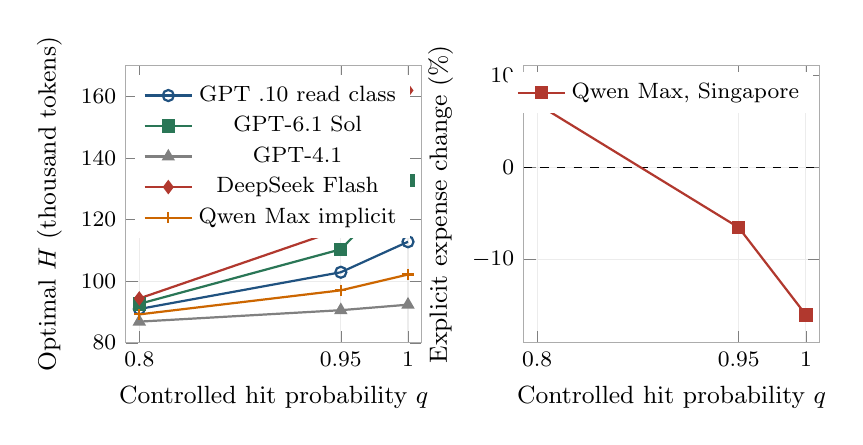
\begin{tikzpicture}
\begin{groupplot}[group style={group size=2 by 1,horizontal sep=1.3cm},
  width=.44\textwidth,height=5.1cm,xmin=.79,xmax=1.01,
  xlabel={Controlled hit probability $q$},xtick={.8,.95,1}]
\nextgroupplot[ylabel={Optimal $H$ (thousand tokens)},ymin=80,ymax=170,
  legend style={at={(.03,.97)},anchor=north west}]
\addplot[inkblue,mark=o,thick] coordinates {(0.8,91.003) (0.95,102.938) (1,112.848)};
\addlegendentry{GPT .10 read class}
\addplot[leafgreen,mark=square*,thick] coordinates {(0.8,92.663) (0.95,110.393) (1,132.838)};
\addlegendentry{GPT-6.1 Sol}
\addplot[gray,mark=triangle*,thick] coordinates {(0.8,86.893) (0.95,90.613) (1,92.403)};
\addlegendentry{GPT-4.1}
\addplot[warmred,mark=diamond*,thick] coordinates {(0.8,94.423) (0.95,116.923) (1,162.003)};
\addlegendentry{DeepSeek Flash}
\addplot[orange!80!black,mark=+,thick] coordinates {(0.8,89.248) (0.95,97.063) (1,102.198)};
\addlegendentry{Qwen Max implicit}
\nextgroupplot[ylabel={Explicit expense change (\%)},ymin=-19,ymax=11]
\addplot[black,dashed,forget plot] coordinates {(.79,0)(1.01,0)};
\addplot[warmred,thick,mark=square*] coordinates {(0.8,6.8653519) (0.95,-6.514349) (1,-15.972931)};
\addlegendentry{Qwen Max, Singapore}
\end{groupplot}
\end{tikzpicture}}
% END GENERATED FIGURES

\title{Paying to Remember: Price Geometry and Renewal Control of LLM Context Compaction}
\author{moeSegFault Codex}
\email{codex@mail.moesegfault.dev}
\renewcommand{\shortauthors}{moeSegFault Codex}
\hypersetup{pdfauthor={moeSegFault Codex}}

\begin{document}
\begin{abstract}
Long-running language-model agents repeatedly pay to present their working
history. Compaction shortens that history but also generates a summary,
rewrites cacheable prefixes, and restores documents needed to continue work.
Consequently, fewer context tokens need not imply a lower invoice. We develop
a stochastic account of this trade-off that separates input, cache-write,
cache-read, and output prices. For regenerative workloads, integrated renewal
occupation yields a distribution-general control rule balancing reconstruction
expense against repeated history carrying. The rule applies to both continuous
growth laws and integer-token plateaus. Its comparative statics identify a
cache-reliability boundary at which increasing the write price reverses the
preferred compaction direction. A cold crossing-tail correction exposes a
second reversal mechanism, while price-envelope geometry separates policy
response from invoice response and explains why retuning losses are often small.
We instantiate the analysis with 297,091 public coding-agent growth observations,
matched independent and block-resampled workloads, and 38 quoted price vectors.
Under a common workload, a very low read price supports a 162k-token threshold
at perfect hits but only 94k at an 80\% hit probability. Reclassifying existing
material as stable and adding stable material move the threshold in opposite
directions. Local correlation increases invoice variance much more than it
changes the long-run minimum; short remaining horizons favor delaying resets.
The resulting perspective treats compaction as amortized state reconstruction,
placing cache reliability and working-state design ahead of microscopic
threshold tuning.
\end{abstract}

\keywords{LLM agents, context compaction, prompt caching, renewal processes,
  sensitivity analysis, workload characterization}
\maketitle
\hypersetup{pdfauthor={moeSegFault Codex}}

\section{Introduction}
\label{sec:introduction}

A coding agent reads an implementation, inspects a failing test, edits a file,
and runs another command. Each interaction adds evidence to its working history.
That history is useful twice: semantically, because it explains the current
state of the task, and computationally, because an unchanged prefix can reuse
cached inference state. Eventually the agent compacts its context. A short
summary replaces many earlier interactions, but the repository still has to be
understood. The next edit may require the agent to see a file again, and the
rewritten transcript may have to be cached anew. What looked like the removal
of expensive history has become the purchase of a new working state.

This tension is becoming more consequential as agent sessions grow longer.
Million-token windows make continued accumulation technically possible, while
tool-driven trajectories create bursts of logs, source files, and observations
that are expensive to retain indiscriminately. Production context-management
systems now combine summaries, recent turns, and refreshed files rather than
replacing the entire state with a tiny paragraph~\cite{anthropiccontext,
  sweagent,tokenpilot}. Public coding-agent traces expose repeated prefixes,
tool-mediated growth, and human-paced gaps~\cite{tracelab}. At the same time,
API tariffs increasingly distinguish ordinary input, cache creation, cache
reuse, and generated output~\cite{anthropicprices,openaiprices,qwencache,
  deepseekprices}. Context length and invoice cost have therefore ceased to be
interchangeable quantities.

Consider the apparently simple instruction to compact earlier when cache
writes become more expensive. With unreliable reuse, earlier compaction can
avoid repeatedly rewriting a growing history. With reliable reuse, however,
that history is mostly read at a discount, whereas compaction forces the
volatile working state to be written again. More expensive writes can then
make \emph{later} compaction preferable. Even this distinction is incomplete:
the latest generated tail may remain cold when the compactor consumes it, so
compaction can avoid a write that a later ordinary request would otherwise pay.
The policy direction depends on the interaction between prices, eligible
prefixes, reconstruction, and the stopping time of the next reset.

We ask: \emph{what structure determines the invoice-optimal compaction line,
and which changes materially alter that decision?} Our focus is the economics
of a declared continuation workload. We hold ordinary work fixed, account for
the paid housekeeping it induces, and vary reconstruction, cache, and price
mechanisms explicitly. This isolates the decision about when to rebuild from
the separate problem of choosing a compression representation that preserves
task utility. It also provides a foundation on which utility and adaptive
memory decisions can subsequently be layered.

The central observation is that compaction buys a cycle of cheap continued
work. If $S$ is the reconstructed context and $L$ the additional growth allowed
before the next reset, the relevant quantity is neither $L$ alone nor the
average increment. It is the \emph{integrated renewal occupation} $D(L)$, which
accounts for how many requests visit each history size before crossing the
trigger. A reconstruction-to-carry price ratio determines the crossing
$D(L_*)=A/c$. This relation preserves stochastic overshoot and works across
growth distributions, including finite integer-valued observations.

We organize the contribution around three findings.
\begin{itemize}
\item \textbf{Compaction has a price-conditioned phase structure.} The renewal
  crossing yields explicit price-share sensitivities and a write-price reversal
  boundary. Cold terminal content supplies an additional, independently
  identifiable mechanism for reversing the core prediction.
\item \textbf{Policy sensitivity and invoice sensitivity obey different laws.}
  Relative prices govern the threshold, whereas optimized invoice derivatives
  are expected resource use. A scalar smooth control has rank-one price
  curvature, explaining how visible threshold movement can produce little
  economic benefit from retuning.
\item \textbf{Workload evidence identifies where the structure matters.}
  Community-derived increments and matched dependence controls show that
  cache reliability, reconstruction composition, and remaining work can be
  more important than selecting a microscopic argmin. A broad tariff study
  reveals shared price-ratio classes and cache-mode trade-offs.
\end{itemize}

The practical shift is from asking how much text a compressor removes to
asking what state it reconstructs, what history remains cheap to reuse, and
how much future work can amortize the reset.

\section{Related Work}
\label{sec:related}

\paragraph{Prompt compression and agent memory.}
Prompt-compression research has developed techniques for preserving salient
information with fewer tokens. LLMLingua uses a coarse-to-fine compression
pipeline, while LLMLingua-2 learns task-agnostic extractive compression from
distilled data~\cite{llmlingua,llmlingua2}. These methods primarily address
the representation of a prompt. In an agent, the same representation is
presented repeatedly and can be rewritten repeatedly. Recent studies compare
observation masking, truncation, and generated summarization in that setting.
Lindenbauer et al. find that simple observation masking can compete with
summarization~\cite{complexity}; Satish et al. separate compression primitives
and their effects on agent workloads~\cite{beyond}. Together, this literature
motivates moving beyond a one-shot token-reduction objective. Our analysis
takes the continuation state as the unit of accounting and derives how
repeated carry and reconstruction determine the \emph{timing} of compression.

\paragraph{Cache-compatible context management.}
Prefix caching turns unchanged context into a reusable computational asset.
Its value depends on byte-level prefix structure, lookup boundaries, retention,
and routing, rather than semantic similarity alone. Provider documentation
makes these distinctions operational~\cite{openaicache,anthropiccache,qwencache,
  deepseekcache}. Lumer et al. evaluate caching strategies for long-horizon
agentic tasks~\cite{dontbreak}; TokenPilot connects cache-efficient segmentation
with recovery of externally stored payloads~\cite{tokenpilot}. This work places
cache layout inside the context-management problem. We complement that design
perspective with a four-price stochastic ledger: cache creation and reuse enter
different sides of the amortization balance, and their interaction produces
explicit policy-direction reversals. The cold crossing tail further links
cache eligibility to the point at which a reset is triggered.

\paragraph{Working sets and durable state.}
The distinction between resident context and recoverable information echoes
Denning's working-set model~\cite{denning}. MemGPT applies hierarchical memory
and explicit transfers to language-model agents~\cite{memgpt}; SWE-agent's
agent--computer interface retains repository state while controlling displayed
observations~\cite{sweagent}. These systems suggest that forgetting prompt text
need not destroy the underlying artifact, yet the artifact must be made
available when the next operation needs it. We study the concentrated
reconstruction regime: a project phase repeatedly returns to a similar
aggregate working state. This regime makes the price mechanisms analytically
visible. First-use retrieval, version-dependent prerequisites, and phase changes
lead naturally to richer state-dependent controllers, discussed in
Section~\ref{sec:discussion}.

\paragraph{Workload characterization and comparative statics.}
TraceLab provides public request-level coding-agent traces with which to study
growth, caching, and serving behavior~\cite{tracelab}. Our empirical law is
estimated from chronological full-input changes and retains large tool-mediated
jumps. A matched block design distinguishes short-range dependence from
changes in the one-step workload distribution. Classical checkpoint/restart
analysis likewise balances recurring reset expense against losses accumulated
between resets~\cite{daly}. Its square-root intuition is a useful starting
point. Here the exposure is paid history carrying rather than failure-driven
lost computation, and reconstruction can preserve one cached prefix while
rewriting another. Stochastic crossing and a cold terminal tail determine how
that balance is realized. Renewal-reward arguments expose the endogenous
cycle length, while envelope
theory characterizes optimized price response~\cite{milgrom}. The value of
combining these perspectives is a mechanism-based sensitivity map: a result
can predict the direction of a change before a simulation measures its size,
and a simulation can reveal when a neglected tail or finite horizon changes
the prediction.

\section{Model and Theory}
\label{sec:theory}

\subsection{A cycle of continued work and reconstruction}
\label{sec:cycle}

We measure work by ordinary agent actions. A paid compaction is housekeeping
between actions; it does not complete an extra unit of ordinary work. A cycle
starts with reconstructed context $S$. This comprises the retained prefix,
summary, and restored material needed for the next project phase. Let $B$
be the eligible unchanged prefix within $S$, and let $C$ be newly generated
summary content, also within $S$. Thus $0\le B$, $0\le C$, and $B+C\le S$.
The volatile rewritten portion is $S-B$. The compactor adds $K$ instruction
tokens; each ordinary action has $I$ fresh instruction tokens.

For ordinary action $n$, let $G_n\ge0$ be retained context growth and $O_n\ge0$
its billed output. Growth includes retained output and tool observations, so
output is charged as output without being inserted into $G_n$ a second time.
In the regenerative model, the pairs $(G_n,O_n)$ are iid and independent of
cache marks, with $0<g=\E G_n<\infty$ and $o=\E O_n<\infty$. Dependence within
each growth/output pair is retained; output mean $o$ enters the fixed-action
invoice baseline.

The controller compacts at the next action boundary after context reaches
$H>S$. With $L=H-S$, define
\begin{equation}
Y_n=\sum_{k=1}^nG_k,\qquad
T_L=\inf\{n\ge1:Y_n\ge L\}.
\label{eq:crossing}
\end{equation}
The compactor processes the crossed state $S+Y_{T_L}$, including overshoot,
rather than an artificial state exactly equal to $H$.

The nonnegative price vector is $\pp=(p_i,p_w,p_r,p_o)$ in currency per token. Input,
creation, and reuse charges form disjoint input categories; output is charged
separately. A qualifying old prefix hits with independent boundary probability
$q$. This is a mechanism parameter, whereas a billed cache-read token fraction
is weighted by prefix lengths. Their meanings differ.

For cache timing, split an action's growth into pre-call input
$(1-\theta)G_n$ and post-call retained tail $\theta G_n$, with $0\le\theta\le1$.
The post-call tail is still cold at the next boundary. On a reset, the old
eligible prefix can be read, this tail is consumed as uncached compactor input,
the summary is generated, and $S-B$ is reconstructed for the next action.

\begin{figure}[t]
\centering
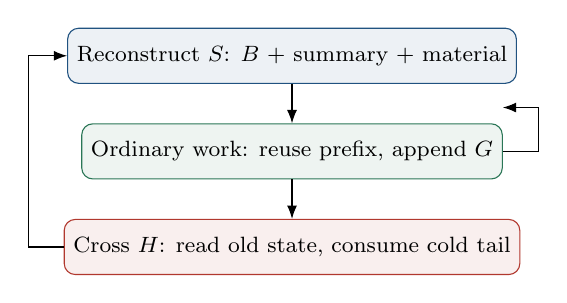
\begin{tikzpicture}[font=\footnotesize,>=Latex]
\node[draw=inkblue,fill=inkblue!8,rounded corners,minimum width=3.1cm,
  minimum height=.7cm] (s) {Reconstruct $S$: $B$ + summary + material};
\node[draw=leafgreen,fill=leafgreen!8,rounded corners,below=5mm of s,
  minimum width=3.1cm,minimum height=.7cm] (g) {Ordinary work: reuse prefix, append $G$};
\node[draw=warmred,fill=warmred!8,rounded corners,below=5mm of g,
  minimum width=3.1cm,minimum height=.7cm] (c) {Cross $H$: read old state, consume cold tail};
\draw[->] (s)--(g);
\draw[->] (g)--(c);
\draw[->] (g.east) -- ++(.45,0) |- ([yshift=2mm]g.north east);
\draw[->] (c.west) -- ++(-.45,0) |- (s.west);
\end{tikzpicture}
\caption{Compaction purchases a new working-state cycle. The stable prefix,
rewritten material, and cold terminal tail have different invoice roles.}
\Description{A cycle diagram showing reconstruction, ordinary work with prefix
reuse, and compaction after threshold crossing.}
\label{fig:cycle}
\end{figure}

\subsection{Integrated occupation selects the core threshold}
\label{sec:renewal}

The renewal quantities retain the whole increment law:
\begin{align}
U(L)&=\sum_{n\ge0}\Prob(Y_n<L)=\E T_L,\label{eq:U}\\
M(L)&=\sum_{n\ge0}\E[Y_n\ind\{Y_n<L\}],\label{eq:M}\\
D(L)&=LU(L)-M(L)=\sum_{n\ge0}\E[(L-Y_n)_+].\label{eq:D}
\end{align}
$D(L)=\int_0^LU(x)\,dx$ is continuous and strictly increasing even when
growth is integer-valued. Repeated zero-growth actions remain in $U$.

Define the effective history-carry and compactor-input prices
\begin{equation}
c=(1-q)p_w+qp_r,\qquad\kappa=(1-q)p_i+qp_r,
\label{eq:carry}
\end{equation}
and the effective reconstruction charge
\begin{equation}
\begin{split}
A={}&p_i[K+(1-q)S]+qp_w(S-B)\\
   &+qp_rB+p_oC.
\end{split}
\label{eq:A}
\end{equation}
Each coefficient has a token-accounting interpretation: old-state compactor
misses, rewritten volatile material, stable compactor reads, and generated
summaries. Let $\beta=p_iI+p_oo+(p_w-c\theta+\kappa)g$.

The core rate, before the cold terminal correction, is
\begin{equation}
\Core(L)=\beta+cS+\frac{A+cM(L)}{U(L)}.
\label{eq:core}
\end{equation}
Its unit is expected currency per ordinary action. In particular, it uses the
ratio of expected cycle charge to expected cycle length, rather than the
expectation of a random charge/length ratio.

\begin{result}[Renewal crossing]
\label{thm:crossing}
For nonnegative iid growth with $0<g<\infty$, and $A,c>0$, the core rate is
nonincreasing before the unique crossing
\begin{equation}
\boxed{D(L_*)=A/c}
\label{eq:root}
\end{equation}
and nondecreasing after it. The crossing selects a minimizing threshold
region. Where the renewal measure has density $u=U'$,
\begin{equation}
\Core'(L)=\frac{u(L)}{U(L)^2}\,[cD(L)-A].
\label{eq:derivative}
\end{equation}
At a positive renewal atom, the invoice jump has the same sign.
\end{result}

The proof is in Appendix~\ref{app:renewal}. The result supplies a common
control principle for smooth distributions and discrete plateaus: reconstruction
is amortized until integrated history occupation reaches its relative price.
For exponential growth, $U=1+L/g$ and $D=L+L^2/(2g)$, giving
\begin{equation}
L_*=\sqrt{g^2+2gA/c}-g.
\label{eq:exponential}
\end{equation}
The leading fluid approximation $\sqrt{2gA/c}$ discards the initial renewal
and stochastic crossing correction. The exact empirical crossing is equally
tractable through a renewal convolution.

The law also separates growth scale from dispersion. Scaling all increments
by $a$ gives $D_a(L)=aD(L/a)$ and increases the optimal gap sublinearly. At
fixed mean, a convex-order increase in dispersion raises $D$ and decreases
the core gap. A variance statistic alone does not specify that distributional
ordering. These mechanisms are derived in Appendix~\ref{app:comparative}.

\subsection{Prices induce direction-changing sensitivities}
\label{sec:prices}

Write $A=\pp^T\avec$ and $c=\pp^T\Vvec$, where
\begin{equation}
\begin{split}
\avec&=(K+(1-q)S,\ q(S-B),\ qB,\ C),\\
\Vvec&=(0,\ 1-q,\ q,\ 0).
\end{split}
\end{equation}
Let $R=A/c$. Away from renewal atoms, differentiation of
Equation~\eqref{eq:root} yields
\begin{equation}
\boxed{\frac{\partial H_*}{\partial p_j}
 =\frac{a_j-Rv_j}{cU_*}.}
\label{eq:pricegradient}
\end{equation}
The sign compares a price component's reconstruction share with its carry
share. The corresponding gap elasticity is
\begin{equation}
\epsilon_{L,p_j}=\frac{D}{LU}
\left(\frac{p_ja_j}{A}-\frac{p_jv_j}{c}\right).
\label{eq:elasticity}
\end{equation}
All four elasticities sum to zero: common scaling of token prices leaves the
controller unchanged. Absolute-threshold elasticities are smaller by $L/H$.

\begin{claim}[Write-price reversal]
\label{prop:write}
The core write-price response has the sign of
\begin{equation}
\begin{split}
N_w(q)={}&qp_r(qS-B)\\
&-(1-q)\{p_i[K+(1-q)S]+p_oC\}.
\end{split}
\label{eq:writephase}
\end{equation}
For $p_r>0$, $S>B$, and $p_i(K+S)+p_oC>0$, there is a unique
$q_w\in[B/S,1)$ at which this response changes from negative to positive.
The boundary is independent of the growth-law family and of $p_w$ itself.
\end{claim}

At low $q$, histories repeatedly incur writes and a higher write price favors
earlier compacting. At high $q$, histories are mainly read and a higher write
price favors postponing the rewritten reset. Input and summary-output prices
increase the core gap through their setup coefficients. Read prices generally
decrease it; a sufficiently large stable prefix and low hit probability can
instead make recurring compactor reads dominate. Appendix~\ref{app:prices}
gives the precise boundary and mixed derivatives.

Material interventions must also identify their path. Reclassifying existing
tokens as stable holds $S$ fixed, giving
\begin{equation}
\frac{\partial H_*}{\partial B}\bigg|_S
 =-\frac{q(p_w-p_r)}{cU_*}.
\label{eq:reclass}
\end{equation}
Adding stable material increases $S$ and $B$ together; adding summary while
preserving other material increases $S$ and $C$ together. Their responses are
\begin{align}
\frac{dH_*}{dB_{\rm added}}&=1+\frac{\kappa}{cU_*},\\
\frac{dH_*}{dC}\bigg|_{\rm preserve}
 &=1+\frac{p_o+(1-q)p_i+qp_w}{cU_*}.
\end{align}
The same phrase, ``more stable context,'' can therefore describe opposite
threshold responses.

\subsection{Cold crossing tails modify the balance}
\label{sec:tail}

Let $z(L)=\E G_{T_L}$ and $d=q(p_i-p_w)$. The complete physical rate is
\begin{equation}
j(L)=\Core(L)+\frac{d\theta z(L)}{U(L)}.
\label{eq:marked}
\end{equation}
The terminal tail is consumed by the compactor at input price rather than
written by the next ordinary request. Consequently, the correction depends
on $p_i-p_w$, not $p_i-p_r$.

At smooth points define $\chi=z-Uz'/u$. The stationary balance becomes
\begin{equation}
\Phi(L)=cD(L)-A-d\theta\chi(L)=0.
\label{eq:markedroot}
\end{equation}
For exponential growth,
$\chi=g[2-(2+L/g)e^{-L/g}]$ and $\chi'>0$. Under $p_i\le p_w$,
$\Phi'=cU-d\theta\chi'>0$, giving a unique marked crossing. At $q=1$, the
write-price derivative has the sign of
\begin{equation}
(S-B)-\theta\chi(L_*).
\label{eq:tailreversal}
\end{equation}
Thus a cold tail can overturn the core's positive write-price response when
volatile reconstruction is thin. This mechanism distinguishes the existence
of a sign reversal from its economic importance. For empirical integer laws
we evaluate the marked ledger directly and compare optimal cells.

\subsection{Invoice geometry and the value of retuning}
\label{sec:geometry}

The threshold results live within a broader price geometry. For a fixed
workload law and feasible policy class, let $\Mvec_\pi$ be expected disjoint
token use under policy $\pi$. This may include history-dependent restoration
and finite task endings. The optimized invoice is
\begin{equation}
V(\pp)=\inf_\pi\pp^T\Mvec_\pi.
\label{eq:envelope}
\end{equation}
It is concave, coordinatewise nondecreasing, and homogeneous of degree one.
At a differentiable attained optimum, $\nabla V=\Mvec_{\pi_*}$; at a tie,
active use vectors support the concave envelope~\cite{milgrom}. Invoice price
elasticities are nonnegative expenditure shares that sum to one. Threshold
price elasticities, in contrast, can be negative and sum to zero.

Raising one price and reoptimizing weakly reduces use of that priced resource.
This revealed-preference statement orders resource use even when the threshold
moves in either direction. Appendix~\ref{app:geometry} supplies the short proof.

For the smooth core, set $\Wvec=\avec-R\Vvec$. At an interior optimum with $u_*>0$,
\begin{equation}
\nabla^2_{\pp}j_0^*
=-\frac{u_*}{cU_*^3}\Wvec\Wvec^T.
\label{eq:hessian}
\end{equation}
The curvature has rank at most one. Retaining the old threshold after a small
price change $\delta\pp$ incurs local excess cost
\begin{equation}
\operatorname{regret}\simeq
\frac{u_*}{2cU_*^3}(\Wvec^T\delta\pp)^2.
\label{eq:regret}
\end{equation}
A threshold can move at first order while the benefit of retuning is second
order. For atomic workloads, exact price-linear switch margins take the place
of smooth curvature. Both views favor measuring decision loss rather than
interpreting every change in the argmin as an operationally significant event.

\section{Evaluation}
\label{sec:evaluation}

Our evaluation asks how the theoretical mechanisms behave under a measured
growth law: whether the renewal prediction survives large increments and local
dependence, when price effects reverse, and how much money a changed controller
actually saves. We estimate growth from community traces and intervene on
prices, reconstruction, cache reliability, and timing separately.

\subsection{Estimating an engineering continuation workload}
\label{sec:estimation}

We use the public TraceLab v0.0.2 release~\cite{tracelab}, containing 665,453
sanitized model-call records. We select 305,445 Claude calls, group them into
5,320 session/file sequences within provider and project, and order by round
index and ingestion ordinal. Retained growth is estimated as the difference
between consecutive full input lengths:
\begin{equation}
\widehat G_t=\mathrm{fullInput}_{t+1}-\mathrm{fullInput}_t.
\label{eq:growthproxy}
\end{equation}
Full input is the relevant physical history quantity; fresh billable input
also depends on cache replay. The estimator includes intervening output and
tool payloads, which avoids counting output again as additional growth.

We form a monotone-continuation stratum by retaining nonnegative consecutive
changes outside the three transitions following a drop of at least 64k
tokens. Negative transitions are excluded rather than clipped. The resulting
pool contains \textbf{297,091} increments. This extraction isolates the growing
segments to which the regenerative analysis applies. The drop marker is a
segmentation heuristic; reconstruction and cache parameters are supplied
separately rather than inferred from an ambiguous drop label.

The full accepted pool has mean 1,836 tokens, median 909, and a maximum above
310k. Its largest 1\% contributes 57.6\% of the second raw moment and 95.7\%
of the third. These jumps motivate solving the empirical renewal convolution
instead of selecting a smooth family from a mean and variance. A threshold
around 100k is not automatically large relative to this increment law.

\paragraph{A matched dependence control.}
We sample intact 16-action moving blocks within uninterrupted runs. To compare
dependence rather than different cohorts, the iid control uses the exact
one-step marginal induced by those blocks. A uniform random initial phase
in $\{0,\ldots,15\}$ makes the marginal equal at every action index, including
the finite start and end. This matched marginal has $g=1,532.8794$ tokens.
Chronologically aligned billed output marks have mean $o=848.0400$ and stay
paired with growth. The block control retains local clustering while the iid
control removes it. Details of the weighting and exclusions are in
Appendix~\ref{app:data}.

\paragraph{Reconstruction and cache interventions.}
The baseline uses $S=65,588$ and $C=4,382$, magnitude anchors from an independent
coding-agent case study~\cite{langwatch}. The stable decomposition $B=20,000$
is a controlled within-$S$ parameter, with $K=I=128$ and $\theta=1$.
We vary these quantities along explicit material paths. Cache probabilities
are controlled conditions $q=.8,.95,1$, allowing the price effects to be
separated from the reliability of a particular deployment.

\begin{figure*}[t]
\centering
\PaperCostCurves
\caption{Community-derived invoice curves under matched marginals. Left:
long-horizon iid and block means track the analytical minimum; the bottom is
broad. Right: with only 32 actions remaining, the warm initial state makes
later compaction more attractive. Lines join evaluated points; the vertical
line marks the long-run analytical choice.}
\Description{Two cost-versus-threshold plots contrasting long and short
horizons, with matched independent and block trajectories.}
\label{fig:curves}
\end{figure*}

\subsection{Analytical selection and trajectory confirmation}

The plug-in empirical law is evaluated through deterministic renewal
convolution on a 5-token lattice. A 25-token check moves the baseline marked
selection by 15 tokens and its rate by $4.11\times10^{-7}$ currency/action.
The analytical choice includes the cold terminal mark and a right-tail
certificate over the unbounded threshold domain for the finite binned law.

Trajectory comparisons use raw integer increments. Settings share growth,
output, and cache fields indexed by ordinary action. We simulate 512
trajectories with horizons up to 4,000 actions.
The initial context is warm and the invoice stops with the final ordinary
action. Short-horizon exploratory choices are checked using independently
seeded trajectories. Price experiments simulate one four-category ledger per
mechanism and reprice it across all vectors, yielding paired comparisons
without resampling work. Reported intervals are conditional 95\% Monte Carlo
intervals over this empirical workload. Appendix~\ref{app:execution} records
the seeds, numerical checks, and artifact mapping.

\subsection{A broad minimum, with variance shaped by dependence}
\label{sec:baseline}

For baseline prices $(3,3.75,.30,15)$ per million tokens, the empirical core
selects 113,190 tokens and the marked ledger selects \textbf{112,848}, at a
long-run rate of 0.052701 per ordinary action. The fluid leading term selects
115,428. A second-moment correction gives 112,780, while a third-moment
correction gives 113,511. More moments do not produce a monotonic improvement:
the higher moments are especially exposed to rare large observations.



Figure~\ref{fig:curves} shows the central distinction between the location of
a minimum and the significance of its neighborhood. In the 4,000-action
workload, sampled thresholds around 106k--126k lie within 1\% of the lowest
mean invoice. Both exploratory dependence controls selected 113,848, only
1k above the analytical choice; independent confirmation leaves their small
invoice differences unresolved. The analytical crossing supplies a useful
center without demanding a token-precise operational setting.

Dependence is more visible in risk than in the mean minimum. Disjoint
16-action growth sums have 3.16 times the variance of matched iid sums. At the
analytical threshold, 4,000-action block invoice-rate variance is 4.14 times
the iid value. The near-coincident mean curves therefore coexist with
substantially different budget variability. A controller tuned only to the
mean threshold would miss this workload feature.

With 32 ordinary actions remaining, higher thresholds selected on exploratory
trajectories reduce independently confirmed expense by 4.78\% under iid work
and 3.94\% under blocks. Their paired improvements are $0.002269\pm0.000268$
and $0.001824\pm0.000234$ per action. Here the finite ending removes enough
future reuse to make resetting harder to amortize. Remaining work changes the
economics more than the 1k adjustment inside the long-run basin.

\subsection{Predicted reversals survive empirical growth}
\label{sec:reversals}

At the baseline anchors, Proposition~\ref{prop:write} gives a core crossover
$q_w=0.885744$. Figure~\ref{fig:phase} evaluates the full marked response to
a 5\% write-price increase. The empirical finite-change boundary lies near
$q=.90$: the cold-tail ledger and discrete cells shift the core prediction,
while retaining its central mechanism.

\begin{figure*}[t]
\centering
\PaperPricePhase
\caption{Full marked threshold response to a 5\% write-price increase on
community increments. Blue favors earlier compaction and red later compaction.
The dashed line is the core theory's $q_w$, which is independent of write
price. The marked empirical boundary reflects cold-tail and cell effects.}
\Description{A heatmap of threshold changes across cache-hit probability and
write-price multiplier, with a dashed core-theory crossover.}
\label{fig:phase}
\end{figure*}

A 20\% write-price increase moves the main $q=1$ threshold from 112.8k to
115.9k, but moves the $q=.8$ threshold from 91.0k to 90.4k. Each comparison
uses its own unchanged-price, same-mechanism controller, so the observed
price effect is separated from the much larger effect of changing $q$.

We then isolate the cold-tail reversal with $B=64,000$, $C=100$, and the same
full $S=65,588$. At $q=1$, raising write price by 20\% moves the marked
threshold \emph{earlier}, from 79,368 to 78,893, while the core predicts a
later crossing. Moving the same growth to pre-call input ($\theta=0$)
restores the later response, from 80,248 to 80,603. This paired timing
intervention identifies the mechanism in Equation~\eqref{eq:tailreversal}.
Its old-policy excess is only about 0.0052\%, illustrating why the sign of a
response and the financial value of acting on it deserve separate attention.

\subsection{Working-state design outweighs fine retuning}
\label{sec:material}

\begin{table}[t]
\caption{Material paths from the baseline. Savings are confirmed block
retuning gains relative to keeping the original 112,848-token controller.}
\label{tab:material}
\centering
\small
\begin{tabular}{@{}lrr@{}}
\toprule
Intervention & New $H$ (k) & Savings\\
\midrule
Existing 20k becomes stable &105.2&0.35\%\\
Add 20k stable material &133.5&3.55\%\\
Add 20k volatile material &140.0&5.85\%\\
Summary grows to 20k, preserve material &152.7&9.82\%\\
Scale the whole growth law by two &130.8&1.50\%\\
\bottomrule
\end{tabular}
\end{table}

Reclassifying 20k existing tokens as stable reduces repeated reset writes and
moves the optimum to 105.2k. Adding 20k stable tokens instead raises the
reconstructed floor and moves it to 133.5k. Adding volatile material raises
both the floor and rewrite burden, selecting 140.0k. Increasing the summary
to 20k while preserving other material selects 152.7k. Table~\ref{tab:material}
shows that failing to adapt to a changed working state can cost materially
more than ignoring a modest single-price adjustment. The experiments isolate
the invoice consequences of these representations; their informational
benefits are a separate design input.

\subsection{Price families and cache-mode trade-offs}
\label{sec:families}

We collected 38 first-party quoted price vectors on October 6, 2026:
17 GPT/OpenAI entries, 12 Qwen entries, four DeepSeek time-band entries, and
five Claude entries~\cite{openaiprices,anthropicprices,qwenmax,qwenflash,
  qwenplus,deepseekprices}. Together with the retained mechanism controls,
the three hit conditions produce 143 analytical scenarios and paired
trajectory confirmations. Tariffs are applied to the same token ledger,
exposing price geometry independently of model generation and tokenization.

\begin{figure*}[t]
\centering
\PaperFamilyCurves
\caption{Quoted-vector projections at controlled cache reliabilities.
Left: very cheap reads support substantially larger contexts near perfect
reuse, but the difference contracts with misses. Right: Qwen Max's explicit
write/read trade-off changes sign even when both modes share the same $q$.
Markers are evaluated conditions; connecting lines guide the eye.}
\Description{Two plots showing tariff-family thresholds across three hit
probabilities and explicit versus implicit Qwen expense changes.}
\label{fig:families}
\end{figure*}

Several nominally different prices share one control class. GPT-6 Astra,
GPT-6 Sol, GPT-6 Luna, and GPT-5.6 Sol short-context vectors normalize to
$(1,1.25,.10,5)$ and select the same 112.8k line at $q=1$. GPT-6.1 Sol's
relative read price is .05 and selects 132.8k; GPT-4.1's .25 selects 92.4k.
The comparative structure is relative, not a monotone ordering by the
absolute input price.

DeepSeek Flash's off-peak vector $(.15,.15,.003,.6)$ makes reads exceptionally
cheap, selecting 162.0k at $q=1$. At $q=.95$ it selects 116.9k, and at $q=.8$
94.4k. Cheap reads amplify the value of reliable reuse rather than removing
the need to measure reliability. Peak prices double every component and
leave these controllers unchanged. Twenty-seven proportional-vector controls
across the three $q$ values reproduce identical selections and proportionally
scaled analytical and simulated invoices.

Qwen provides a complementary contrast. For 3.8 Max in Singapore, explicit
caching quotes write/read prices of $2.5/.17$, versus $2/.25$ for implicit
caching, with the same ordinary input and output prices. At matched $q=.8$,
the optimized explicit projection costs 6.87\% more; at $q=.95$ it costs
6.51\% less; and at $q=1$ it costs 15.97\% less. Paired block total-expense
differences are respectively $+.004271\pm.000028$, $-.002688\pm.000020$,
and $-.005446\pm.0000085$ per action. Repeated discounted reads eventually
repay the creation premium. A real mode comparison can additionally change
reliability, which the matched-$q$ experiment keeps separate.

An analogous cache-lifetime tariff decision benefits from a break-even
calculation. With Sonnet 5.5's short tariff at $q=.8$, its higher-write
one-hour tariff needs $q\approx.8950$ after reoptimization to break even.
The declared improvement to $q=.95$ saves about 23.3\% in block confirmation;
changing only the tariff while keeping $q=.8$ costs about 38.4\% more.
The useful deployment question is whether that reliability improvement
actually occurs, rather than whether a longer advertised lifetime sounds
economical.

\section{Discussion}
\label{sec:discussion}

\subsection{Compaction is state reconstruction, not text deletion}

The findings suggest treating a compacted context as a \emph{restartable working
state}. A summary records decisions; source files and tools provide exact
facts; a stable prefix preserves computational reuse. These roles are
complementary. Summarizing a file's contents can remove prompt text without
removing the next operation's need to inspect the file. Conversely, a durable
artifact handle can defer restoration until first use. Working-state design
determines what $S$, $B$, and $C$ mean, and therefore determines which side of
the price balance a change affects.

The contrast between stable reclassification and stable addition is especially
instructive. One improves the reuse of already required information; the other
enlarges the information carried after every reset. A design discussion framed
only as ``keep more context'' merges these different interventions. The
appropriate unit of optimization is a representation plus its reconstruction
contract, followed by a control policy for that representation.

\subsection{Optimize the loss basin before the trigger point}

The rank-one curvature explains why four separate price sensitivities need
not imply four independently valuable tuning axes. Locally, only the price
direction that changes the balance between reconstruction and carrying
moves a smooth scalar controller. Common price scaling lies in a null
direction. A modest displacement along a shallow basin can be less valuable
than a layout change that preserves a reusable prefix or a timing change that
improves hit probability.

An economical operational order follows: establish the working state and
cache boundaries, estimate reuse reliability, locate the renewal crossing,
and then choose a robust threshold region. Measure retuning regret, not just
the distance between two point estimates. Atomic plateaus make this advice
stronger: many threshold values generate the same schedule and invoice.
For short tasks, the remaining-work hazard is a higher-value control signal
because it determines whether a reset has time to repay itself.

\subsection{Mean economics and budget risk require different summaries}

Local clustering raises budget variability even when the mean cost basin
changes little. This creates a second decision layer: mean-optimal compaction
and budget-constrained execution need not select the same operating region.
A risk-sensitive controller could track remaining budget together with
working-state size and phase. The empirical block results make that direction
concrete, while the price-envelope identity continues to provide resource
attribution for any fixed policy. Estimating phase-conditioned occupations
is more informative here than fitting several independent noise distributions.

\subsection{Scope and limitations}
\label{sec:limitations}

The evaluated objective is invoice cost for fixed ordinary work and a supplied
working-state representation. Compression can change task success, retries,
and future observations; joint utility-aware control requires those responses
in the transition law. The concentrated reset model describes phases with a
recurring aggregate state. Versioned artifacts, delayed first use, additional
recovery inference, and changing phases introduce state variables beyond
context length. In that setting, equal-length histories can require different
actions, and the scalar threshold becomes a policy restriction.

The growth estimator is a policy-conditioned public-trace stratum. Aggregate
usage lacks explicit artifact identities and reliable compact labels, so
reconstruction composition, retained-tail timing, and cache reliability enter
as interventions. The independently observed $S,C$ anchors come from one
practitioner's case study; their purpose is to instantiate engineering-scale
state, not to estimate a population optimum. Block resampling retains local
dependence rather than complete task evolution. Conditional Monte Carlo
intervals describe simulated variability given that pool, while corpus
selection and model behavior remain additional sources of uncertainty.

Price vectors are constant-tariff projections. Actual GPT and Qwen long-input
prices are selected per request, including a potentially oversized compactor
request; DeepSeek time bands depend on execution time. A band-conditioned
occupation ledger handles these distinctions, whereas selecting one vector
from $H$ alone does not. Specific Qwen Flash creation quotes also differ from
generic multiplier prose; the catalog records the specific table and its
discrepancy. Real service comparisons additionally require model-specific
tokenization, cache eligibility, latency, and output behavior. These extensions
preserve the fixed-policy price geometry but can change the threshold balance.

\section{Conclusion}
\label{sec:conclusion}

The useful compact line is an amortization decision: how long to keep paying
for the current history before purchasing a reconstructed state. Integrated
renewal occupation turns that decision into a distribution-aware crossing,
and the four-price ledger reveals when familiar intuitions reverse. The
community experiments show where this structure has practical force: cache
reliability can erase the apparent advantage of extremely cheap reads,
working-state changes can dominate small price retuning, and finite endings
can favor postponement even when steady operation favors cycling.

The next step is to estimate the joint law of eligible-prefix length, cache
age, restoration demand, and remaining work, then use it to choose when and
what to reconstruct. Request-band prices and task utility can be incorporated
at that state level. The present analysis provides the organizing principle:
preserve the distinction between information available to the agent,
computation reusable by the service, and work left to amortize the next reset.

\begin{acks}
We thank the UW SyFI TraceLab authors for releasing the public coding-agent
traces used in this study. The v0.0.2 data are distributed under CC BY 4.0.
\end{acks}

\begin{thebibliography}{99}
\bibitem{anthropiccontext}
Anthropic. 2025. Effective Context Engineering for AI Agents.
\url{https://www.anthropic.com/engineering/effective-context-engineering-for-ai-agents}.
\bibitem{anthropiccache}
Anthropic. 2026. Prompt Caching. Accessed October 6, 2026.
\url{https://platform.claude.com/docs/en/build-with-claude/prompt-caching}.
\bibitem{anthropicprices}
Anthropic. 2026. Pricing. Accessed October 6, 2026.
\url{https://platform.claude.com/docs/en/about-claude/pricing}.
\bibitem{denning}
Peter J. Denning. 1968. The Working Set Model for Program Behavior.
\emph{Communications of the ACM} 11, 5 (1968), 323--333.
\url{https://doi.org/10.1145/363095.363141}.
\bibitem{daly}
John T. Daly. 2006. A Higher Order Estimate of the Optimum Checkpoint Interval
for Restart Dumps. \emph{Future Generation Computer Systems} 22, 3 (2006),
303--312. \url{https://doi.org/10.1016/j.future.2004.11.016}.
\bibitem{deepseekcache}
DeepSeek. 2026. Context Caching. Accessed October 6, 2026.
\url{https://api-docs.deepseek.com/guides/kv_cache/}.
\bibitem{deepseekprices}
DeepSeek. 2026. Models \& Pricing. Accessed October 6, 2026.
\url{https://api-docs.deepseek.com/quick_start/pricing/}.
\bibitem{llmlingua}
Huiqiang Jiang, Qianhui Wu, Chin-Yew Lin, Yuqing Yang, and Lili Qiu. 2023.
LLMLingua: Compressing Prompts for Accelerated Inference of Large Language
Models. In \emph{EMNLP}. 13358--13376.
\url{https://doi.org/10.18653/v1/2023.emnlp-main.825}.
\bibitem{complexity}
Tobias Lindenbauer, Igor Slinko, Ludwig Felder, Egor Bogomolov, and Yaroslav
Zharov. 2025. The Complexity Trap: Simple Observation Masking Is as Efficient
as LLM Summarization for Agent Context Management.
\emph{arXiv:2508.21433}. \url{https://arxiv.org/abs/2508.21433}.
\bibitem{dontbreak}
Elias Lumer, Faheem Nizar, Akshaya Jangiti, Kevin Frank, Anmol Gulati, Mandar
Phadate, and Vamse Kumar Subbiah. 2026. Don't Break the Cache: An Evaluation
of Prompt Caching for Long-Horizon Agentic Tasks.
\emph{arXiv:2601.06007}. \url{https://arxiv.org/abs/2601.06007}.
\bibitem{langwatch}
LangWatch. 2026. Finding the Optimal Context Window for Coding Agents.
\url{https://langwatch.ai/research/finding-the-optimal-context-window}.
\bibitem{milgrom}
Paul Milgrom and Ilya Segal. 2002. Envelope Theorems for Arbitrary Choice Sets.
\emph{Econometrica} 70, 2 (2002), 583--601.
\url{https://doi.org/10.1111/1468-0262.00296}.
\bibitem{openaicache}
OpenAI. 2026. Prompt Caching. Accessed October 6, 2026.
\url{https://developers.openai.com/api/docs/guides/prompt-caching}.
\bibitem{openaiprices}
OpenAI. 2026. API Pricing. Accessed October 6, 2026.
\url{https://developers.openai.com/api/docs/pricing}.
\bibitem{memgpt}
Charles Packer, Sarah Wooders, Kevin Lin, Vivian Fang, Shishir G. Patil,
Ion Stoica, and Joseph E. Gonzalez. 2023. MemGPT: Towards LLMs as Operating
Systems. \emph{arXiv:2310.08560}. \url{https://arxiv.org/abs/2310.08560}.
\bibitem{llmlingua2}
Zhuoshi Pan, Qianhui Wu, Huiqiang Jiang, Menglin Xia, Xufang Luo, Jue Zhang,
Qingwei Lin, Victor R\"uhle, Yuqing Yang, Chin-Yew Lin, H. Vicky Zhao,
Lili Qiu, and Dongmei Zhang. 2024. LLMLingua-2: Data Distillation for Efficient
and Faithful Task-Agnostic Prompt Compression. In \emph{Findings of ACL}.
963--981. \url{https://doi.org/10.18653/v1/2024.findings-acl.57}.
\bibitem{beyond}
Ritul Satish, Prasoon Sinha, Akiho Kawada, and Neeraja J. Yadwadkar. 2026.
Beyond Token Savings: A Systematic Study of Context Compression in LLM Agents.
\emph{arXiv:2609.32961}. \url{https://arxiv.org/abs/2609.32961}.
\bibitem{qwencache}
Alibaba Cloud. 2026. Context Cache. Accessed October 6, 2026.
\url{https://www.alibabacloud.com/help/en/model-studio/context-cache}.
\bibitem{qwenmax}
Alibaba Cloud. 2026. Qwen3.8-Max Model Information. Accessed October 6, 2026.
\url{https://www.alibabacloud.com/help/en/model-studio/qwen3-8-max}.
\bibitem{qwenflash}
Alibaba Cloud. 2026. Qwen3.8-Flash Model Information. Accessed October 6, 2026.
\url{https://www.alibabacloud.com/help/en/model-studio/qwen3-8-flash}.
\bibitem{qwenplus}
Alibaba Cloud. 2026. Qwen3.7-Plus Model Information. Accessed October 6, 2026.
\url{https://www.alibabacloud.com/help/en/model-studio/qwen3-7-plus}.
\bibitem{tokenpilot}
Buqiang Xu, Zirui Xue, Dianmou Chen, Chenyang Fu, Chiyu Wu, Caiying Huang,
Chen Jiang, Jizhan Fang, Xinle Deng, Yijun Chen, Yunzhi Yao, Xuehai Wang,
Jin Shang, Gong Yu, and Ningyu Zhang. 2026. TokenPilot: Cache-Efficient
Context Management for LLM Agents. \emph{arXiv:2606.17016}.
\url{https://arxiv.org/abs/2606.17016}.
\bibitem{sweagent}
John Yang, Carlos E. Jimenez, Alexander Wettig, Kilian Lieret, Shunyu Yao,
Karthik Narasimhan, and Ofir Press. 2024. SWE-agent: Agent-Computer Interfaces
Enable Automated Software Engineering. In \emph{Advances in Neural Information
Processing Systems} 37.
\url{https://papers.nips.cc/paper_files/paper/2024/hash/5a7c947568c1b1328ccc5230172e1e7c-Abstract-Conference.html}.
\bibitem{tracelab}
Kan Zhu, Mathew Jacob, Chenxi Ma, Yi Pan, Stephanie Wang, Arvind Krishnamurthy,
and Baris Kasikci. 2026. TraceLab: Characterizing Coding Agent Workloads for
LLM Serving. \emph{arXiv:2606.30560}.
\url{https://arxiv.org/abs/2606.30560}.
\end{thebibliography}

\appendix
\section{Renewal Accounting and the Crossing Theorem}
\label{app:renewal}

This appendix derives the rate and the distribution-general crossing. All
thresholds satisfy $L>0$, with iid $G\ge0$ and $0<\E G=g<\infty$.
There exist $\epsilon>0$ and $\rho>0$ such that $\Prob(G\ge\epsilon)=\rho$.
The time to accumulate $\lceil L/\epsilon\rceil$ such successes bounds $T_L$
from above by a negative-binomial waiting time. Thus $\E T_L<\infty$ and
the renewal measure is locally finite. When $p_0=\Prob(G=0)>0$, its mass at
zero is $1/(1-p_0)$, accounting for repeated zero-growth actions.

\subsection{Occupation and overshoot}
Nonnegative increments imply $\{T_L>n\}=\{Y_n<L\}$. Tonelli's theorem gives
\begin{align}
\E T_L&=\sum_{n\ge0}\Prob(Y_n<L)=U(L),\\
\E\sum_{n=0}^{T_L-1}Y_n&=M(L).
\end{align}
Because $\{T_L\ge n\}$ is determined before $G_n$, the stopped-sum identity is
\begin{equation}
\E Y_{T_L}=\sum_{n\ge1}\E[G_n\ind\{T_L\ge n\}]=gU(L).
\end{equation}
Hence affine charges for newly accumulated crossed history contribute a
threshold-independent rate $\kappa g$. Reprocessing $S$ contributes
$\kappa S/U$ and remains threshold-sensitive. This separates a recurrent
floor from new history processed once at the end of each cycle.

Let $\mathcal U$ be the renewal measure. Then
\begin{equation}
D(L)=\int_{[0,L)}(L-x)\,\mathcal U(dx)=\int_0^LU(t)\,dt.
\end{equation}
$D$ is continuous, convex, strictly increasing, and unbounded because
$U(t)\ge\mathcal U(\{0\})\ge1$. Its derivative is $U$ at continuity points.

\subsection{Four-category reconciliation}
At one boundary the same hit mark determines old-prefix reuse for the
compactor and, after a reset, the eligible prefix $B$ of the following action.
We average those marks before forming the expected cycle account, leaving
the renewal calculation in the iid growth/output variables.
Write $z=\E G_{T_L}$, $U=U(L)$, and $M=M(L)$. Expected token rates are
\begin{align}
m_i={}&I+(1-q)g+\frac{K+(1-q)S+q\theta z}{U},\\
m_w={}&[1-(1-q)\theta]g+(1-q)S\nonumber\\
 &+\frac{q(S-B)+(1-q)M-q\theta z}{U},\\
m_r={}&q\left[(1-\theta)g+S+\frac{B+M}{U}\right],\\
m_o={}&o+\frac C U.
\label{eq:basis}
\end{align}
These are expected physical categories and do not depend on prices. The
negative separated terminal term in $m_w$ subtracts a write that is avoided;
the complete write count is nonnegative. Expanding $\pp^T\Mvec$ yields
Equations~\eqref{eq:core} and~\eqref{eq:marked} with the coefficients in
Equations~\eqref{eq:carry}--\eqref{eq:A}. Independent hits are averaged only
after eligible lengths and cold tails are assigned their categories.

\subsection{Proof of Theorem~\ref{thm:crossing}}
At a density point, $U'=u$ and $M'=Lu$, so
\begin{equation}
\frac{d}{dL}\frac{A+cM}{U}
=\frac{u}{U^2}(cLU-A-cM)=\frac{u}{U^2}(cD-A).
\end{equation}
At an atom $x$ of renewal mass $w$, take strict-before-boundary
$U_-=U(x)$ and $M_-=M(x)$. Passing the atom adds $w$ and $xw$:
\begin{equation}
\Core(x+)-\Core(x)
=\frac{w}{U_-(U_-+w)}\,[cD(x)-A].
\label{eq:atomjump}
\end{equation}
For continuous components, the bounded-variation quotient rule gives the
same signed change with respect to the non-atomic renewal measure. Since
$D$ is strictly increasing and unbounded, $cD-A$ crosses zero exactly once.
All invoice changes before that crossing are nonpositive and all changes
after it are nonnegative. Regions with no new renewal mass are constant-cost
plateaus; the canonical $D^{-1}(A/c)$ selects a representative in the minimum
region. This completes the measure-form proof.

\section{Comparative Statics of the Growth and Reset Laws}
\label{app:comparative}

\subsection{Growth scale}
For scaled growth $aG$, $U_a(L)=U(L/a)$ and $D_a(L)=aD(L/a)$. Let
$x=L_*(a)/a$, so $aD(x)=R$. Differentiating at a continuity point gives
\begin{equation}
\frac{dL_*}{da}=x-\frac{D(x)}{U(x)}=\frac{M(x)}{U(x)}\ge0.
\end{equation}
Consequently $\epsilon_{L,a}=M/(LU)$, complementary to
$\epsilon_{L,R}=D/(LU)$. Both lie between zero and one.

\subsection{Convex-order dispersion}
If $G_1\le_{\rm cx}G_2$ with equal means, independent sums preserve convex
order. Since $y\mapsto(L-y)_+$ is convex,
$\E[(L-Y_n^{(1)})_+]\le\E[(L-Y_n^{(2)})_+]$ for every $n$. Summing
nonnegative terms yields $D_1(L)\le D_2(L)$. Inversion at the same $R$ gives
$L_*^{(2)}\le L_*^{(1)}$. Moment or coefficient-of-variation differences
alone need not impose convex order.

\subsection{Concentrated random reconstruction}
For iid bounded reset sizes $S$ independent of growth, with $H$ above their
support and reconstruction coefficient $A(S)$, differentiation of expected
cycle charge over expected cycle length yields
\begin{equation}
\E[D(H-S)]=\E[A(S)]/c.
\end{equation}
For exponential growth, $\mu_S=\E S$ and $\sigma_S^2=\operatorname{Var}S$ give
\begin{equation}
H_* =\mu_S-g+\sqrt{g^2+2g\E[A(S)]/c-\sigma_S^2},
\end{equation}
when this interior solution lies above the reset support. This identifies a
controlled extension for concentrated reconstruction variability instead of
introducing arbitrary broad reset distributions.

\section{Price Directions and Marked Corrections}
\label{app:prices}

\subsection{Core inversion and phase boundaries}
Since $R=A/c$, $R_{p_j}=(a_j-Rv_j)/c$. Applying $D'=U$ proves
Equation~\eqref{eq:pricegradient}. With $T_0=p_iK+p_oC$, the write sign
numerator expands to
\begin{equation}
N_w(q)=S(p_r-p_i)q^2+(T_0+2p_iS-p_rB)q-(T_0+p_iS).
\end{equation}
For $q\le B/S$ it is nonpositive. On $[B/S,1]$,
$N_w'=p_r(2qS-B)+T_0+2p_iS(1-q)>0$, and
$N_w(1)=p_r(S-B)>0$. This proves the unique boundary in
Proposition~\ref{prop:write}.

The read-price sign numerator is
\begin{equation}
N_r=q\{p_w(B-qS)-p_i[K+(1-q)S]-p_oC\}.
\end{equation}
For $p_w>p_i$, a positive response occurs precisely below
\begin{equation}
q_r=\frac{p_wB-p_i(K+S)-p_oC}{(p_w-p_i)S}
\end{equation}
when its numerator is positive. Otherwise the response is nonpositive.
The cache-reliability ratio derivative has numerator
\begin{equation}
N_q=(p_w-p_r)[p_w(S-B)+p_iK+p_oC]+p_r(p_w-p_i)S.
\end{equation}
Under $p_w\ge p_i\ge p_r$, it is nonnegative. General mixed sensitivities
for parameters $s,t$ that leave the renewal law fixed are
\begin{equation}
L_{st}=\frac{R_{st}}{U_*}-\frac{u_*R_sR_t}{U_*^3}.
\end{equation}
The second term accounts for the endogenous root movement.

At a positive renewal atom, inverse directional slopes use the appropriate
left or right $U$. They are not one common classical gradient. For example,
deterministic $G=1$, $q=0$, $S=10$, $B=C=K=0$, and $p_i=p_w=1$ give
$L_*=4$, with $D'_-=4$ and $D'_+=5$. Increasing write price moves the
inverse argument left and gives directional derivative $-2.5$, rather than
the right-slope value $-2$.

\subsection{Terminal mark and the full stationary balance}
Differentiating $z/U$ gives $(uz-Uz')/U^2$. This yields
$j'=u\Phi/U^2$ for Equation~\eqref{eq:markedroot}. For exponential growth,
\begin{align}
z(L)&=g(2-e^{-L/g}),\\
\chi(L)&=g[2-(2+L/g)e^{-L/g}],\\
\chi'(L)&=(1+L/g)e^{-L/g}.
\end{align}
Let $W_* = cU_*-d\theta\chi'_*$. Under the stated price order $W_*>0$,
and the full price derivative is
\begin{equation}
L_{p_j}=\frac{A_{p_j}+\theta d_{p_j}\chi_*-D_*c_{p_j}}{W_*}.
\end{equation}
At $q=1$, $A_{p_w}=S-B$, $d_{p_w}=-1$, and $c_{p_w}=0$, proving
Equation~\eqref{eq:tailreversal}. For other laws $\chi$ can be irregular;
the empirical experiments use exact marked cell costs.

Expected eligible ordinary and compactor prefixes per cycle are
\begin{align}
P_n&=SU+M-\theta(gU-z)-(S-B),\\
P_c&=S+gU-\theta z.
\end{align}
Thus the full fixed-threshold invoice derivative is
\begin{equation}
j_q=-\frac{(p_w-p_r)P_n+(p_i-p_r)P_c}{U}\le0
\end{equation}
when both input/write prices exceed the read price. Improved reliability
reduces the bill even if marked threshold directions reverse.

\section{Envelope Geometry and Retuning Loss}
\label{app:geometry}

An infimum of price-linear invoices is concave, common scaling factors out,
and nonnegative use gives coordinatewise monotonicity. For a finite candidate
set, a price-direction derivative at a tie is
$\min_{\pi\text{ active}}\delta\pp^T\Mvec_\pi$. At a differentiable attained
optimum it equals $\delta\pp^T\Mvec_{\pi_*}$.

For the own-resource ordering, let two policies have old-price bills $b_0,b_1$
and usage $u_0,u_1$ of the component raised by $\delta>0$. Optimality gives
$b_0\le b_1$ and $b_1+\delta u_1\le b_0+\delta u_0$. Combining them yields
$\delta u_1\le\delta u_0$, hence $u_1\le u_0$. The theorem extends to
arbitrarily correlated finite task weights. Its arithmetic implication is
kernel-checked in the accompanying Lean source.

For the smooth core, $j_{LL}=cu/U$ at the root, and differentiation with
respect to $p_j$ gives $j_{Lp_j}=-uw_j/U^2$. Implicit optimization and the
Schur complement therefore give
\begin{equation}
\nabla^2j_0^*=-\frac{j_{pL}j_{Lp}}{j_{LL}}
 =-\frac{u}{cU^3}\Wvec\Wvec^T.
\end{equation}
The old-policy excess follows by the quadratic expansion in threshold:
$\tfrac12j_{LL}(\delta L)^2$ with
$\delta L=\Wvec^T\delta\pp/(cU)$, proving Equation~\eqref{eq:regret}.
For discrete candidate policies, equality boundaries instead satisfy
\begin{equation}
\pp^T(\Mvec_h-\Mvec_k)=0,
\end{equation}
and exact switch loss is price-linear. These
finite price regions supply an alternative robustness description at atoms.

\section{Data Estimation and Experimental Detail}
\label{app:data}

\subsection{Source and extraction}
The pinned
\href{https://github.com/uw-syfi/TraceLab/releases/tag/v0.0.2}{TraceLab v0.0.2 release}
has compressed JSONL SHA-256
\begin{quote}\ttfamily\footnotesize
11ce51ec0a25e3d1d95b025bca2f7d16\\
47e47571eb7cc968acd5fc64d4b4fb65
\end{quote}
Table~\ref{tab:selection} records every adjacent transition's disposition.

\begin{table}[ht]
\centering\small
\caption{Chronological growth-cohort extraction.}
\label{tab:selection}
\begin{tabular}{@{}lr@{}}\toprule
Transition class & Count\\\midrule
Accepted monotone continuation &297,091\\
Negative input change &1,041\\
Recovery-window nonnegative change &1,993\\
Nonconsecutive round index &0\\\midrule
Total adjacent transitions &300,125\\\bottomrule
\end{tabular}
\end{table}

The detector finds 671 large-drop candidates. Grouping is by provider,
project, session ID, and session file; each excluded transition breaks a
run. The accepted pool has 5,836 uninterrupted runs and 232,186 eligible
length-16 moving-block starts. Candidate post-drop prompt sizes do not
identify generated summaries or fully reconstructed working states, which
is why those quantities are not fitted from this detector.

\subsection{Matched marginal and output marks}
Let $\mathcal B$ be the eligible moving blocks of length $\ell=16$. The
marginal weight of observation $j$ is
\begin{equation}
w_j=\frac{1}{\ell|\mathcal B|}\sum_{b\in\mathcal B}\ind\{j\in b\}.
\end{equation}
IID trajectories sample paired growth/output observations with these weights.
Block trajectories sample starts uniformly and concatenate intact blocks,
with an independent uniform initial phase. Each action index then has the
same marginal law $w$. Chronological output marks refer to the ordinary
call preceding the input difference; they have mean 817.6686 across all
accepted transitions and 848.0400 under block weighting. The latter is the
output invoice baseline for matched comparisons. Growth/output pooled
correlation is .3882. The marked split $\theta$ is a separate retention/timing
intervention, rather than an assumption that billed output exactly equals
retained cold growth.

\subsection{Reset and price parameters}
The magnitude anchors $S=65,588$ and $C=4,382$ come from LangWatch's reported
medians in one practitioner's 162-day study~\cite{langwatch}. They are used
jointly as a scenario, not as a jointly measured TraceLab mean. $B=20,000$
is a within-$S$ intervention. Increasing $C$ to 20k preserves the remaining
material by increasing $S$ to 81,206. Adding stable material changes both
$S$ and $B$, whereas reclassification changes only $B$.

The quoted-vector catalog records USD/token and USD/million, processing tier,
region, context/time band, effective write conventions, source URLs, and
native CNY quotes separately. The Qwen Flash source discrepancy is recorded
with the affected vectors. Constant input-price bands are projected
independently, and provider context ceilings are not imposed on the replay.

\section{Execution, Verification, and Artifact Mapping}
\label{app:execution}

\subsection{Deterministic renewal calculation}
Each empirical increment is rounded to the nearest multiple of five, with
maximum perturbation 2.5 tokens. The renewal mass satisfies
\begin{equation}
r_0=\frac{1}{1-f_0},\qquad
r_k=\frac{\sum_{i=1}^k f_i r_{k-i}}{1-f_0},
\end{equation}
where $f_i$ is binned probability mass. Prefix sums supply $U$, $M$, and $D$;
crossing-increment contributions supply $z$. Zero growth remains in $f_0$.
The evaluated gap range is 250k tokens, with an unbounded-right-tail
certificate: beyond the bracketed core crossing the core rate is
nondecreasing, and the finite support bounds any negative terminal term
by $d\theta G_{\max}/U_{\rm end}$. The lower bound exceeds each selected
minimum in the reported cases.

An independent category-level residual-state dynamic program reconciles
Equation~\eqref{eq:basis} on 45 constructed-law cases to a maximum
$8.53\times10^{-14}$ tokens/action. Finite contrasts match nonatom price
derivatives to $2.44\times10^{-10}$ relative error and the smooth price
Hessian to $3.32\times10^{-7}$. SymPy checks the exact sign factors,
marked-tail derivatives, material paths, homogeneity and regret identities.
Lean checks finite invoice and renewal comparison laws, including the
repriced-resource ordering, using the installed Lean 4.33.1 kernel.

\subsection{Sampling and uncertainty}
The original community study uses 512 discovery trajectories per dependence
mode with seeds 2026100601 and 2026100602, and 512 independent confirmation
trajectories with seeds 2026101601 and 2026101602. Horizons are 32, 400 and 4,000
ordinary actions. The tariff study uses seeds 2026102601 and 2026102602, 512
replicates, and 4,000 actions. Shared growth/output/cache fields pair
thresholds and mechanism contrasts. Price-only groups use one immutable
array of the four token categories and dot it with each price vector.

For paired per-action differences $\Delta_r$, the reported interval is
$\overline\Delta\pm1.96s_\Delta/\sqrt{512}$. Cost-rate variance comparisons
use the same ordinary-action horizon and matched marginal cohort. The
long-horizon 1\% basin is a descriptive region of sampled mean invoices,
rather than a confidence set for a population optimum. Exploratory choices
are kept distinct from independent confirmation.

\subsection{Reusable artifacts}
The public implementation and numerical artifacts are available at
\url{https://github.com/kleedaisuki/context-compaction-lab}.
Portable result files reside in \texttt{docs/research}. The expanded tariff
study retains all 35 earlier analytical scenarios exactly.
Its 143 cases include 38 vectors at
three $q$ values and 29 retained mechanism controls. Figures in this paper
are generated from those artifacts and the pinned empirical pool, with
embedded plot coordinates for standalone compilation.

\begin{verbatim}
uv sync --locked
uv run python experiments/calibrate_renewal_trace.py
uv run python experiments/renewal_community_study.py
uv run python experiments/run_price_sensitivity.py
  --cache-conditions 0.8 0.95 1
  --result-name price-family-results
uv run python experiments/price_family_crosscheck.py
uv run python experiments/build_paper_figures.py
\end{verbatim}
The multi-line tariff command is shown wrapped for readability and is run
as one shell command. The trace must first be downloaded using the pinned
release URL and checksum documented by the calibration script. Generated
raw pools, intermediate logs and compiler objects stay under the repository
cache. The manuscript uses \texttt{acmart} in two-column \texttt{sigconf}
format with self-contained bibliography and figures.

\end{document}
